% !TEX program = xelatex
\documentclass[UTF8,fontset=fandol,a4paper,11pt]{ctexart}
\usepackage[margin=21mm,top=23mm,bottom=22mm,headheight=16pt]{geometry}
\usepackage{amsmath,amssymb,mathtools,bm}
\usepackage{tikz}
\usetikzlibrary{arrows.meta,calc,angles,quotes,patterns,decorations.pathmorphing}
\usepackage{xcolor,booktabs,array,longtable,enumitem,fancyhdr,needspace}
\usepackage[unicode,hidelinks]{hyperref}
\definecolor{ink}{HTML}{24343C}
\definecolor{accent}{HTML}{166A70}
\definecolor{muted}{HTML}{65747A}
\definecolor{rulegray}{HTML}{D4DDE0}
\definecolor{warm}{HTML}{966037}
\color{ink}
\setlength{\parindent}{2em}
\setlength{\parskip}{4pt}
\linespread{1.12}
\AtBeginDocument{\setlength{\abovedisplayskip}{6pt plus 2pt minus 1pt}
\setlength{\belowdisplayskip}{6pt plus 2pt minus 1pt}
\setlength{\abovedisplayshortskip}{0pt plus 1pt}
\setlength{\belowdisplayshortskip}{4pt plus 1pt}}
\setlist[enumerate]{label=(\arabic*),leftmargin=2.3em,itemsep=3pt,topsep=4pt}
\setlist[itemize]{leftmargin=2em,itemsep=2pt,topsep=4pt}
\allowdisplaybreaks[1]
\setlength{\emergencystretch}{2em}
\setcounter{secnumdepth}{0}
\providecommand{\tightlist}{\setlength{\itemsep}{0pt}\setlength{\parskip}{0pt}}
\ctexset{section={format=\Large\bfseries\color{accent},beforeskip=10pt,afterskip=9pt},
subsection={format=\normalsize\bfseries\color{accent},beforeskip=10pt,afterskip=4pt},
subsubsection={format=\normalsize\bfseries,beforeskip=8pt,afterskip=3pt}}
\pagestyle{fancy}
\fancyhf{}
\fancyhead[L]{\small\color{muted}物理学难题集萃}
% 页眉仅保留书名；版本名称只在封面显示。
\fancyfoot[L]{\small\color{muted}\chapterlabel}
\fancyfoot[R]{\small\thepage}
\renewcommand{\headrulewidth}{0.4pt}
\renewcommand{\footrulewidth}{0pt}
\newcommand{\dd}{\mathop{}\!\mathrm{d}}
\newcommand{\vect}[1]{\bm{#1}}
\newcommand{\tagline}[1]{\noindent{\small\color{muted}#1}\par}
\newcommand{\result}[1]{\begin{equation*}\boxed{#1}\end{equation*}}
\newcommand{\figcaption}[1]{\par\vspace{2pt}{\small\color{muted}#1}\par}
\newcommand{\teach}[2]{\Needspace{4\baselineskip}\subsection*{讲解要点与追问}#1\par\smallskip\noindent\textbf{追问：}#2\par}
\newcommand{\workarea}{\par\vspace{7mm}\noindent{\small\color{muted}作答区}\par\vspace{4mm}
\noindent\textcolor{rulegray}{\rule{\linewidth}{0.3pt}}\par\vspace{16mm}
\noindent\textcolor{rulegray}{\rule{\linewidth}{0.3pt}}\par\vspace{16mm}
\noindent\textcolor{rulegray}{\rule{\linewidth}{0.3pt}}\par\vspace{16mm}
\noindent\textcolor{rulegray}{\rule{\linewidth}{0.3pt}}}
\tikzset{axis/.style={-{Stealth[length=2mm]},thin,color=muted},
motion/.style={-{Stealth[length=2.3mm]},thick,color=accent},
force/.style={-{Stealth[length=2.3mm]},thick,color=warm},
traj/.style={thick,color=accent},guide/.style={dashed,thin,color=muted},
object/.style={thick,color=ink},every node/.style={font=\small}}\renewcommand{\result}[1]{\boxed{#1}}\widowpenalty=10000\clubpenalty=10000\displaywidowpenalty=10000

\newcommand{\chapterlabel}{第七章\quad 振动与波动}
\hypersetup{pdftitle={第七章 振动与波动·学生版},pdfauthor={},pdfsubject={第七章第1--43题}}
\begin{document}
\pdfbookmark[0]{第七章 振动与波动}{cover}
\thispagestyle{empty}
\vspace*{20mm}
\noindent{\Huge\bfseries 物理学难题集萃}\par\vspace{8mm}
\noindent{\LARGE 第七章\quad 振动与波动}\par\vspace{10mm}
\noindent{\Large\color{accent}学生版}\par\vspace{8mm}
\noindent\textcolor{accent}{\rule{\linewidth}{1pt}}\par\vspace{8mm}
\noindent 第 1--43 题\par\vspace{5mm}
\noindent 题目、题图与作答区。\par
\vfill\clearpage
\pdfbookmark[1]{题目目录}{contents}
\section*{题目目录}
\begin{longtable}{@{}>{\color{accent}\bfseries}r p{120mm}@{}}
\toprule 题号 & 题目\\\midrule
1 & 弹簧振子与滑块非弹性碰撞后的振动 \\
2 & 密度线性分层液体中的浮力振动 \\
3 & 两滚轮支承木板的微小振动 \\
4 & 地球贯通隧道中的简谐运动 \\
5 & 斜面上弹簧连接滚动圆柱的振动周期 \\
6 & 直角均匀杆连弹簧的微小摆动 \\
7 & 有质量弹簧振子的等效质量修正 \\
8 & 小孔圆周运动与悬挂重物的耦合振动 \\
9 & 旋转平板上弹簧质点的相对运动 \\
10 & 狭长湖泊湖震的整体振荡模型 \\
11 & 滑块摆系统的轨迹与小角振动 \\
12 & 实心球在球形碗底纯滚动的小振动 \\
13 & 物体在两薄壁圆筒上纯滚的振动 \\
14 & 旋转圆盘导轨中弹簧小球的振动 \\
15 & 圆周弹簧质点受径向轻击后的径向频率 \\
16 & 有限振幅单摆周期的二级近似 \\
17 & 谐振子的相积分与能量频率关系 \\
18 & T形导轨约束细杆的小振动与碰撞 \\
19 & 两质量弹簧系统的相对振动 \\
20 & 缓慢缩短摆长时的振幅变化 \\
21 & 小虫沿刚性摆杆爬行时的频率与振幅 \\
22 & 旋转圆盘支架上摆球的平衡与小振动 \\
23 & 弹性碰撞激发弹簧连接双质点振动 \\
24 & 三球双弹簧系统的特征频率和振型 \\
25 & 两端弹簧支承木板的小振动特征频率 \\
26 & 两个弹簧耦合单摆的简正模式 \\
27 & 六球环形弹簧链的特征频率 \\
28 & 圆周弹簧质点链的简正模式与频带 \\
29 & 带阻尼器摆的等效阻尼振动 \\
30 & 临界阻尼是否最快回到平衡位置 \\
31 & 容器振动驱动下的阻尼受迫振子 \\
32 & 受周期外力三滑块弹簧链的响应 \\
33 & 地震波在地幔地芯模型中的传播 \\
34 & 夜间声速梯度导致的声线弯曲 \\
35 & 海洋声道中的声波传播路径 \\
36 & 有质量弹簧中的纵向弹性波 \\
37 & 拉紧弦中简谐波的平均能流 \\
38 & 弦线上附加质点对波的反射 \\
39 & 拍频与空气柱共振测声速 \\
40 & 小提琴弦按点与变线密度的驻波 \\
41 & 两列反向横波叠加的驻波能量 \\
42 & 飞机越顶飞行的多普勒频移测高 \\
43 & 圆周运动音叉的多普勒频率极值 \\
\bottomrule\end{longtable}


\clearpage
% STUDY_GUIDE_BEGIN
\section*{本章学习安排}
先备知识是受力与力矩方程、机械能、质心和转动惯量。第1--15题先练习选取独立位移，在平衡位置展开到二阶能量；第16--22题再处理有限振幅、缓慢变参和旋转参考系，区分精确式与小量近似。第23--28题进入耦合振动，先求正常模态，再由初始条件定振幅；第29--32题讨论阻尼与受迫响应，第33--43题转入波动、传播与边界。

每题先在题图上标出正方向、平衡位置与约束，再写运动方程；查阅解答时核对有效质量、恢复系数及舍去项的阶数。湖震题须比较模型与数据，声道题须在数值候选角之后检查上下边界，不能只核对最后一个数值。涉及本征值或连续介质时，可先用能量与量纲估计量级，再读完整推导。
% STUDY_GUIDE_END
\clearpage

\pdfbookmark[2]{第 1 题 弹簧振子与滑块非弹性碰撞后的振动}{q1}

\section*{第 1 题\quad 弹簧振子与滑块非弹性碰撞后的振动}

\tagline{M-07-01}

如图7.1,质量为\(m\)、劲度系数为\(k\)的弹簧振子放在光滑的水平面上,其平衡位置在\(O\)点,其圆频率\(\omega=0.5\pi\ \mathrm{rad}\cdot\mathrm{s}^{-1}\).另一质量亦为\(m\)的质点放在光滑曲面的\(A\)点,\(AB\)间高度差\(h=0.20\ \mathrm{m}\),质点由\(A\)点滑到\(B\)点所需时间\(t_{\mathrm{AB}}=1.5\ \mathrm{s}\),\(OB\)之间的距离\(l=6.0\ \mathrm{m}\).现将弹簧振子向左压缩到\(x_{0}=2.0\ \mathrm{m}\)处自由释放,同时释放\(A\)处的质点\(m\),两个质点相遇作完全非弹性碰撞后粘在一起,发生碰撞时弹簧作用力可略.若从碰撞开始计时,试求系统振动的数学表达式.(取\(g=10\ \mathrm{m/s}^{2}\)).

\begin{center}\begin{minipage}{\linewidth}\centering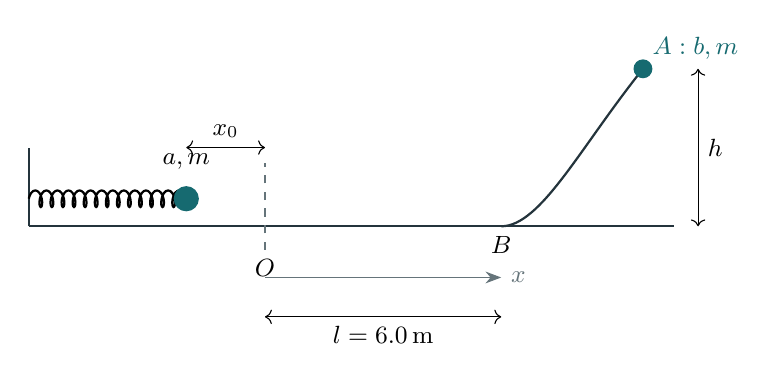
\begin{tikzpicture}[font=\small,spring/.style={decorate,decoration={coil,aspect=.45,segment length=4pt,amplitude=3pt},thick}]
\draw[object](-1,0)--(7.2,0);\draw[object](-1,0)--(-1,1);
\draw[spring](-1,.35)--(1,.35);\fill[accent](1,.35)circle(.16);\node[above]at(1,.6){$a,m$};
\draw[guide](2,-.3)--(2,.8);\node[below]at(2,-.3){$O$};
\draw[object](5,0)..controls(5.5,0)and(6,1)..(6.8,2);
\fill[accent](6.8,2)circle(.12)node[above right]{$A:b,m$};\node[below]at(5,0){$B$};
\draw[<->](1,1)--(2,1)node[midway,above]{$x_0$};
\draw[<->](2,-1.15)--(5,-1.15)node[midway,below]{$l=6.0\,\mathrm m$};
\draw[axis](2,-.65)--(5,-.65)node[right]{$x$};
\draw[<->](7.5,0)--(7.5,2)node[midway,right]{$h$};
\end{tikzpicture}\figcaption{图 7.1}\end{minipage}\end{center}

\workarea

\clearpage

\pdfbookmark[2]{第 2 题 密度线性分层液体中的浮力振动}{q2}

\section*{第 2 题\quad 密度线性分层液体中的浮力振动}

\tagline{M-07-02}

如图,某液体的密度随深度线性地增加,液体表面的密度为\(\rho_{0}\),深度为\(D\)处的密度为\(2\rho_{0}\),一密度为\(2\rho_{0}\)的小球在深度为\(\frac{D}{2}\)处从静止释放.忽略液体的阻力.试求小球的振动表达式.

小球尺度远小于密度变化长度；密度规律在运动所达深度内成立，忽略液体附加质量。

\begin{center}\begin{minipage}{\linewidth}\centering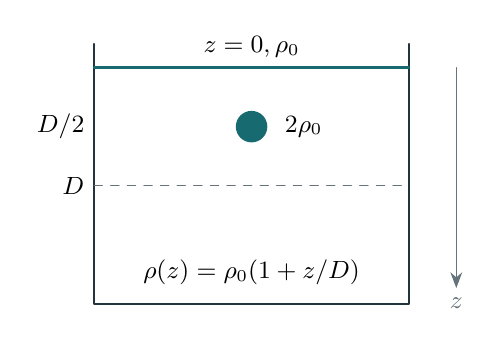
\begin{tikzpicture}[line cap=round,line join=round,spring/.style={decorate,decoration={coil,aspect=.45,segment length=4pt,amplitude=3pt},thick}]\draw[object] (0,3)--(0,-.3)--(4,-.3)--(4,3);\draw[traj] (0,2.7)--(4,2.7);\node[above] at (2,2.7) {$z=0,\rho_0$};\draw[axis] (4.6,2.7)--(4.6,-.1) node[below] {$z$};\draw[guide](0,1.2)--(4,1.2);\node[left]at(0,1.2){$D$};\fill[accent] (2,1.95) circle (.2);\node[right] at (2.3,1.95) {$2\rho_0$};\node[left] at (0,1.95) {$D/2$};\node at (2,.1) {$\rho(z)=\rho_0(1+z/D)$};\end{tikzpicture}\figcaption{图 7.2}\end{minipage}\end{center}

\workarea

\clearpage

\pdfbookmark[2]{第 3 题 两滚轮支承木板的微小振动}{q3}

\section*{第 3 题\quad 两滚轮支承木板的微小振动}

\tagline{M-07-03}

如图7.3,两个完全相同的圆柱状滚轮在水平面内平行放置,各绕自身的轴线按图示方向等角速转动,两轴线之间的距离为\(2l\).在两滚轮上平放一块重量为\(G\)的均匀木板,木板与滚轮之间的摩擦系数为\(\mu\).若木板重心偏离两轴中心位置一个微小的距离,试描述木板的运动.

左轮顶面向右、右轮顶面向左。木板视为薄板，微小振动时两接触始终滑动且摩擦方向保持不变。

\begin{center}\begin{minipage}{\linewidth}\centering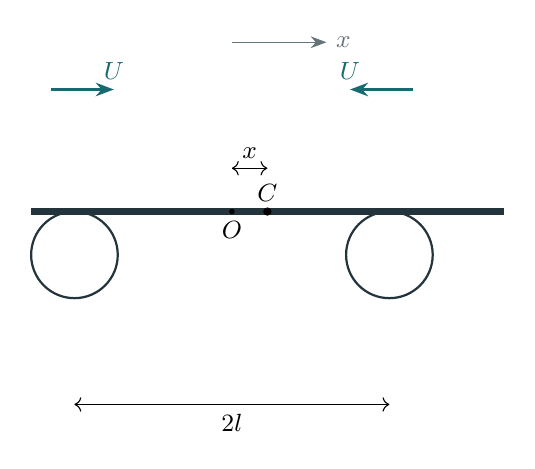
\begin{tikzpicture}[font=\small]
\draw[object,fill=white](0,0)circle(.55);\draw[object,fill=white](4,0)circle(.55);
\draw[object,line width=2.5pt](-.55,.55)--(5.45,.55);
\fill(2.45,.55)circle(1.5pt)node[above]{$C$};\fill(2,.55)circle(1pt)node[below]{$O$};
\draw[motion](-.3,2.1)--(.5,2.1)node[above]{$U$};
\draw[motion](4.3,2.1)--(3.5,2.1)node[above]{$U$};
\draw[axis](2,2.7)--(3.2,2.7)node[right]{$x$};
\draw[<->](0,-1.9)--(4,-1.9)node[midway,below]{$2l$};
\draw[<->](2,1.1)--(2.45,1.1)node[midway,above]{$x$};
\end{tikzpicture}\figcaption{图 7.3}\end{minipage}\end{center}

\workarea

\clearpage

\pdfbookmark[2]{第 4 题 地球贯通隧道中的简谐运动}{q4}

\section*{第 4 题\quad 地球贯通隧道中的简谐运动}

\tagline{M-07-04}

牛顿曾证明:一个均匀球壳,对球壳内物质的万有引力为零,而对球壳外物质的万有引

力不为零,并且其作用就相当于球壳的质量都集中到球心那样(参看力学第三章题11).如图所示,设想沿地球直径开凿一条贯通地球的隧道,将一小球从洞口由静止释放,试求小球到达隧道另一洞口所用的时间.已知地球的半径为\(R\),质量为\(M\),设地球的质量均匀分布.

忽略地球自转、空气阻力及开凿对质量分布的影响。

\begin{center}\begin{minipage}{\linewidth}\centering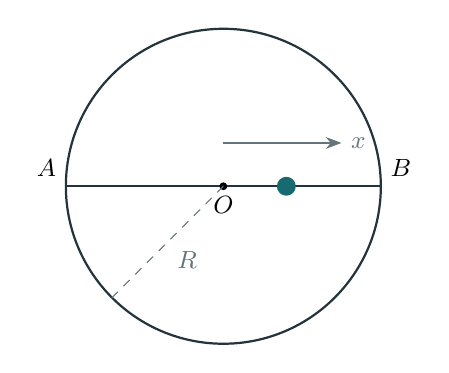
\begin{tikzpicture}[line cap=round,line join=round,spring/.style={decorate,decoration={coil,aspect=.45,segment length=4pt,amplitude=3pt},thick}]\draw[object] (0,0) circle (2);\draw[object] (-2,0)--(2,0);\fill[accent] (.8,0) circle (.12);\fill (0,0) circle (.05);\draw[axis] (0,.55)--(1.5,.55) node[right] {$x$};\node[below] at (0,0) {$O$};\node[above left] at (-2,0) {$A$};\node[above right] at (2,0) {$B$};\draw[guide] (0,0)--(-1.414213562,-1.414213562) node[midway,below right] {$R$};\end{tikzpicture}\figcaption{图 7.4}\end{minipage}\end{center}

\workarea

\clearpage

\pdfbookmark[2]{第 5 题 斜面上弹簧连接滚动圆柱的振动周期}{q5}

\section*{第 5 题\quad 斜面上弹簧连接滚动圆柱的振动周期}

\tagline{M-07-05}

如图7.5,在倾角为\(\theta\)的斜面上有一劲度系数为\(k\)的弹簧,一端固定,另一端与质量为\(m\)的实心圆柱体的轴连接,圆柱体在斜面上作纯滚动.忽略轴承的摩擦.试求振动周期.

\begin{center}\begin{minipage}{\linewidth}\centering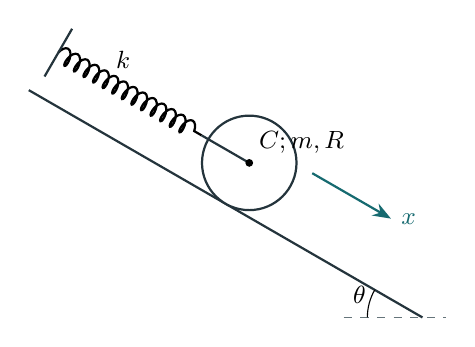
\begin{tikzpicture}[font=\small,spring/.style={decorate,decoration={coil,aspect=.45,segment length=4pt,amplitude=3pt},thick}]
\coordinate(P)at(.5,-.288675135);\coordinate(C)at(.8,.230940108);\coordinate(S)at(-1.624871131,1.630940108);\coordinate(E)at(.193782217,.580940108);
\draw[object](-2,1.154700538)--(3,-1.732050808);\draw[guide](2,-1.732050808)--(3.3,-1.732050808);
\draw[object,fill=white](C)circle(.6);\draw[spring](S)--(E);\draw[object](E)--(C);
\draw[object](-1.799871131,1.327831217)--(-1.449871131,1.934048999);
\fill(C)circle(1.4pt);\node[above right]at(C){$C;m,R$};\node[above]at(-.8,1.3){$k$};
\draw[motion](1.6,.1)--(2.6,-.477350269)node[right]{$x$};
\draw(2.3,-1.732050808)arc(180:150:.7);\node at(2.2,-1.45){$\theta$};
\end{tikzpicture}\figcaption{图 7.5}\end{minipage}\end{center}

\workarea

\clearpage

\pdfbookmark[2]{第 6 题 直角均匀杆连弹簧的微小摆动}{q6}

\section*{第 6 题\quad 直角均匀杆连弹簧的微小摆动}

\tagline{M-07-06}

如图,直角形均匀细杆的水平杆长为\(l\)、质量为\(m\),竖直杆长为\(2l\)、质量为\(2m\),细杆可绕拐角处的固定轴\(O\)无摩擦地转动.水平杆的一端与劲度系数为\(k\)的弹簧相连,平衡时水平杆呈

水平状态,竖直杆竖直下垂．试求微小摆动的周期．

弹簧上端固定在水平杆端点的正上方；只计算微小摆动的一阶回复力矩。

\begin{center}\begin{minipage}{\linewidth}\centering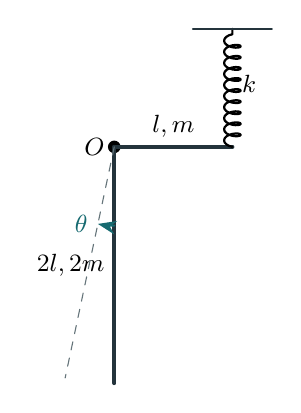
\begin{tikzpicture}[line cap=round,line join=round,spring/.style={decorate,decoration={coil,aspect=.45,segment length=4pt,amplitude=3pt},thick}]\fill (0,0) circle (.08);\node[left] at (0,0) {$O$};\draw[object,line width=1.5pt] (0,0)--(1.5,0);\draw[object,line width=1.5pt] (0,0)--(0,-3);\draw[spring] (1.5,0)--(1.5,1.5);\draw[object] (1,1.5)--(2,1.5);\node[right] at (1.5,.8) {$k$};\node[above] at (.75,0) {$l,m$};\node[left] at (0,-1.5) {$2l,2m$};\draw[guide] (0,0)--(-.623735073,-2.934442802);\draw[motion] (0,-1) arc[start angle=-90,end angle=-102,radius=1] node[left] {$\theta$};\end{tikzpicture}\figcaption{图 7.6}\end{minipage}\end{center}

\workarea

\clearpage

\pdfbookmark[2]{第 7 题 有质量弹簧振子的等效质量修正}{q7}

\section*{第 7 题\quad 有质量弹簧振子的等效质量修正}

\tagline{M-07-07}

如图7.7,弹簧振子中的小球质量为\(M\),弹簧的劲度系数为\(k\),弹簧的质量不可忽略,设为
\(m\),假定弹簧的质量分布均匀,忽略摩擦力.试求振动周期.

先采用长波、同相的近似运动形状，说明等效质量结果的适用条件。

\begin{center}\begin{minipage}{\linewidth}\centering\begin{tikzpicture}[font=\small,line cap=round,spring/.style={decorate,decoration={coil,aspect=.45,segment length=4pt,amplitude=3pt},thick}]
\draw[object](0,-.5)--(0,2.4);\draw[spring](0,2)--(4,2);\draw[object,dashed](4,1.7)rectangle(4.7,2.3);\node at(4.35,2){$M$};
\draw[spring](0,0)--(4.7,0);\draw[object,fill=white](4.7,-.3)rectangle(5.4,.3);\node at(5.05,0){$M$};
\draw[guide](4,-.8)--(4,2.3);\draw[<->](0,2.75)--(4,2.75)node[midway,above]{$L$};
\draw[motion](4,-.8)--(4.7,-.8)node[midway,below]{$u(L,t)$};
\draw[axis](0,1.1)--(4.35,1.1)node[right]{材料坐标$x$};\node[below]at(0,1.1){$0$};\node[below]at(4,1.1){$L$};
\node[right]at(5,2){未形变参考};\node[right]at(5.6,0){瞬时位置};\node[above]at(2,.3){$m,\ k$};
\end{tikzpicture}\figcaption{图 7.7}\end{minipage}\end{center}

\workarea

\clearpage

\pdfbookmark[2]{第 8 题 小孔圆周运动与悬挂重物的耦合振动}{q8}

\section*{第 8 题\quad 小孔圆周运动与悬挂重物的耦合振动}

\tagline{M-07-08}

如图,一不可伸长的细线穿过光滑桌面上的小孔,一端系质量为\(m\)的小球,另一端系质

量为 \(M\) 的重物．小球在桌面上以角速度 \(\omega_{0}\)
作匀速圆周运动，重物静止不动．若重物受到竖直向上或向下的扰动．试证明，重物将作上、下的简谐振动，并求振动圆频率．

扰动位移远小于原圆轨道半径，细线始终绷紧。

\begin{center}\begin{minipage}{\linewidth}\centering\begin{tikzpicture}[font=\small]
\begin{scope}[shift={(-2,0)}]
\draw[guide](0,0)circle(1.4);\fill(0,0)circle(1.2pt)node[below left]{$O$};
\draw[object](0,0)--(1.4,0);\fill[accent](1.4,0)circle(1.8pt)node[right]{$m$};
\draw[motion](1.315569670,.478828201)arc(20:85:1.4);\node[above]at(1.5,1){$\omega_0$};
\node[below]at(.7,0){$r_0$};\node at(0,2.1){俯视：未扰动圆轨道};
\end{scope}
\begin{scope}[shift={(3,0)}]
\draw[object](-1.6,0)--(1.9,0);\draw[object](0,0)--(0,-1.8);\draw[object](0,0)--(1.4,0);
\fill[accent](1.4,0)circle(1.8pt)node[above right]{$m$};\fill(0,0)circle(1pt)node[above left]{$O$};
\fill[accent](0,-1.8)circle(2.3pt)node[left]{$M$};
\draw[<->](0,.65)--(1.4,.65)node[midway,above]{$r$};
\draw[<->](-.55,0)--(-.55,-1.8)node[midway,left]{$l-r$};
\node at(.4,2.1){侧视：绳长约束};
\end{scope}
\end{tikzpicture}\figcaption{图 7.8}\end{minipage}\end{center}

\workarea

\clearpage

\pdfbookmark[2]{第 9 题 旋转平板上弹簧质点的相对运动}{q9}

\section*{第 9 题\quad 旋转平板上弹簧质点的相对运动}

\tagline{M-07-09}

如图7.9,光滑的水平平板绕铅垂轴Oz逆时针作匀角速转动,角速度为\(\omega\).在板面上,一质量可略、原长为\(l\)、劲度系数为\(k\)的弹簧一端固定在O点,另一端系一质量为\(m\)的小球.开始时小球位于\((x_0,0)\),初速度为\((v_0,0)\).试求小球相对平板的运动方程\(x=x(t)\),\(y=y(t)\).

给出的初速度为相对地面的速度；平板坐标轴在初始时与地面轴重合。小球运动限于弹簧长度保持正值的区间。

\begin{center}\begin{minipage}{\linewidth}\centering\begin{tikzpicture}[font=\small,spring/.style={decorate,decoration={coil,aspect=.45,segment length=4pt,amplitude=3pt},thick}]
\draw[guide](0,0)circle(2.2);\draw[axis](-.3,0)--(2.9,0)node[right]{$X=x$};
\draw[axis](0,-.3)--(0,2.8)node[above]{$Y=y$（初始）};
\draw[spring](0,0)--(1.7,0);\fill(0,0)circle(1pt)node[below left]{$O$};
\fill[accent](1.7,0)circle(2pt)node[above]{$m$};
\draw[motion](1.230224387,1.82388266)arc(56:105:2.2)node[left]{$\omega$};
\draw[motion](1.7,-.4)--(2.5,-.4)node[right]{$v_0$（地面）};
\draw[<->](0,-.85)--(1.7,-.85)node[midway,below]{$x_0$};
\end{tikzpicture}\figcaption{图 7.9}\end{minipage}\end{center}

\workarea

\clearpage

\pdfbookmark[2]{第 10 题 狭长湖泊湖震的整体振荡模型}{q10}

\section*{第 10 题\quad 狭长湖泊湖震的整体振荡模型}

\tagline{M-07-10}

狭长、较浅的湖泊可出现湖震，即水体的长周期整体振荡。这里采用矩形容器和平面液面的近似模型，描述水体的长波整体振荡。

我们用一只矩形容器作模型．容器的长度为\(L\)，水高为\(h\)．假定水面开始时与水平面成一小角度．水面开始振荡，振荡时水面仍保持平面，只是绕位于容器长度一半处的水平轴作振荡．

试建立水运动的模型,并求出振荡周期 \(T\) 的表达式.
初始右端液面升高\(\xi\)、左端降低\(\xi\)，从静止开始振荡。 假定
\(\xi \ll h\).

2.下面两个表显示在两种不同长度的容器中,不同深度的水

的振荡时间．以适当的方法检查你得出的公式，看它是否与实验数据很好吻合，并说明你对这种
物理模型的适用性的意见．

表 1 \(L=479 \mathrm{mm}\)

{\def\LTcaptype{none} % do not increment counter
\begin{longtable}[]{@{}ll@{}}
\toprule\noalign{}
h /mm & T /s \\
\midrule\noalign{}
\endhead
\bottomrule\noalign{}
\endlastfoot
30 & 1.78 \\
50 & 1.40 \\
69 & 1.18 \\
88 & 1.08 \\
107 & 1.00 \\
124 & 0.91 \\
142 & 0.82 \\
\end{longtable}
}

表 2 \(L=143 \mathrm{mm}\)

{\def\LTcaptype{none} % do not increment counter
\begin{longtable}[]{@{}ll@{}}
\toprule\noalign{}
$h/\mathrm{mm}$ & \(T/s\) \\
\midrule\noalign{}
\endhead
\bottomrule\noalign{}
\endlastfoot
31 & 0.52 \\
38 & 0.48 \\
58 & 0.43 \\
67 & 0.35 \\
124 & 0.28 \\
\end{longtable}
}

瑞典 Vattern 湖的北端 Bastedalen 与南端 Jonköping
分别测量了湖震时的液面变化。 该湖长度为 123 km,平均深度为 50 m.
在此情况下,时间标度应是什么?

\begin{center}\begin{minipage}{\linewidth}\centering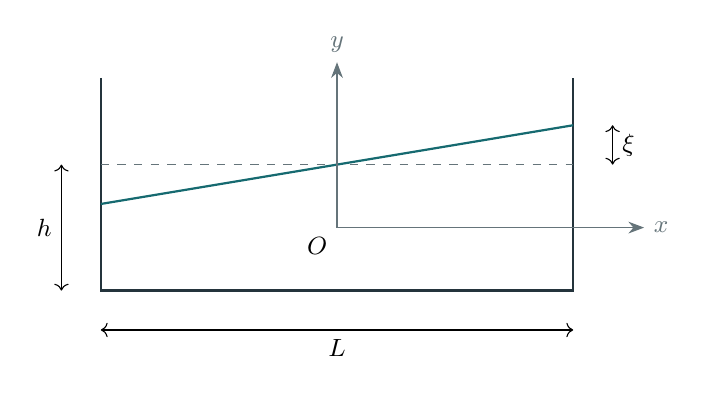
\begin{tikzpicture}[font=\small]
\draw[object](-3,1.7)--(-3,-1)--(3,-1)--(3,1.7);
\draw[guide](-3,.6)--(3,.6);\draw[traj](-3,.1)--(3,1.1);
\draw[<->](3.5,.6)--(3.5,1.1)node[midway,right]{$\xi$};
\draw[<->](-3.5,-1)--(-3.5,.6)node[midway,left]{$h$};
\draw[<->](-3,-1.5)--(3,-1.5)node[midway,below]{$L$};
\draw[axis](0,-.2)--(0,1.9)node[above]{$y$};
\draw[axis](0,-.2)--(3.9,-.2)node[right]{$x$};\node[below left]at(0,-.2){$O$};
\end{tikzpicture}\figcaption{图 7.10}\end{minipage}\end{center}
\begin{center}\begin{minipage}{.97\linewidth}\centering
\begin{tikzpicture}[x=.75cm,y=.75cm,font=\small]
\begin{scope}[yshift=4.4cm]
\draw[axis] (0,-.45)--(0,4.1) node[above]{记录读数};
\draw[axis] (0,0)--(10.6,0) node[right]{时间};
\foreach \v in {0,10,20}{\draw (0,{\v/5})--(-.1,{\v/5}) node[left]{$\v$};}
\node at (5.2,3.55){Bastedalen};
\draw[traj] plot coordinates{(0.069,3.6667) (0.1034,3.3158) (0.1379,2.693) (0.1724,2.3333) (0.2069,1.7193) (0.2414,1.1579) (0.2759,0.4561) (0.3103,0.6842) (0.3448,0.9123) (0.3793,1.1404) (0.4138,1.3684) (0.4483,1.5965) (0.4828,1.8246) (0.5172,1.6667) (0.5517,1.5789) (0.5862,1.4912) (0.6207,1.2281) (0.6552,1.0702) (0.6897,0.9474) (0.7241,0.807) (0.7586,0.6667) (0.7931,0.5439) (0.8276,0.4035) (0.8621,0.5088) (0.8966,0.5965) (0.931,0.7018) (0.9655,0.7895) (1.0,0.8947) (1.0345,1.0526) (1.069,1.2105) (1.1034,1.386) (1.1379,1.5789) (1.1724,1.7018) (1.2069,1.8596) (1.2414,1.8246) (1.2759,1.7895) (1.3103,1.5439) (1.3448,1.0702) (1.3793,0.5965) (1.4138,0.5965) (1.4483,0.614) (1.4828,0.614) (1.5172,0.7018) (1.5517,0.8772) (1.5862,1.0526) (1.6207,1.2281) (1.6552,1.4035) (1.6897,1.4737) (1.7241,1.5614) (1.7586,1.6316) (1.7931,1.7018) (1.8276,1.7895) (1.8621,1.8596) (1.8966,1.8947) (1.931,1.8772) (1.9655,1.8596) (2.0,1.8421) (2.0345,1.6667) (2.069,1.3684) (2.1034,1.0702) (2.1379,0.7719) (2.1724,0.7018) (2.2069,0.6491) (2.2414,0.5789) (2.2759,0.5789) (2.3103,0.6316) (2.3448,0.7018) (2.3793,0.7544) (2.4138,0.8246) (2.4483,0.8772) (2.4828,0.9474) (2.5172,1.0) (2.5517,1.1053) (2.5862,1.193) (2.6207,1.2982) (2.6552,1.4035) (2.6897,1.5088) (2.7241,1.5965) (2.7586,1.7018) (2.7931,1.7368) (2.8276,1.7719) (2.8621,1.807) (2.8966,1.5965) (2.931,0.9825) (2.9655,0.8596) (3.0,0.7544) (3.0345,0.6842) (3.069,0.5965) (3.1034,0.6667) (3.1379,0.7368) (3.1724,0.7895) (3.2069,0.8596) (3.2414,0.9298) (3.2759,1.0) (3.3103,1.0877) (3.3448,1.1754) (3.3793,1.2632) (3.4138,1.3333) (3.4483,1.4211) (3.4828,1.5088) (3.5172,1.614) (3.5517,1.6667) (3.5862,1.7544) (3.6207,1.8246) (3.6552,1.4737) (3.6897,1.1053) (3.7241,0.7719) (3.7586,0.614) (3.7931,0.4211) (3.8276,0.0877) (3.8621,-0.193) (3.8966,-0.0877) (3.931,-0.0877) (3.9655,0.1579) (4.0,0.2632) (4.0345,0.4386) (4.069,0.6316) (4.1034,0.8421) (4.1379,1.0351) (4.1724,1.0526) (4.2069,0.8596) (4.2414,0.6667) (4.2759,0.4737) (4.3103,0.3158) (4.3448,0.1579) (4.3793,0.0877) (4.4138,-0.1579) (4.4483,-0.0877) (4.4828,0.0877) (4.5172,0.2105) (4.5517,0.3333) (4.5862,0.4211) (4.6207,0.4912) (4.6552,0.5614) (4.6897,0.6316) (4.7241,0.7368) (4.7586,0.7719) (4.7931,0.8421) (4.8276,0.8772) (4.8621,0.8947) (4.8966,0.9123) (4.931,0.9298) (4.9655,0.9474) (5.0,0.9649) (5.0345,0.9825) (5.069,1.0351) (5.1034,0.9474) (5.1379,0.5965) (5.1724,0.4912) (5.2069,0.386) (5.2414,0.2807) (5.2759,0.1754) (5.3103,0.0877) (5.3448,0.1228) (5.3793,0.193) (5.4138,0.2456) (5.4483,0.3158) (5.4828,0.3684) (5.5172,0.4561) (5.5517,0.5789) (5.5862,0.7018) (5.6207,0.8246) (5.6552,0.9474) (5.6897,1.0) (5.7241,0.9825) (5.7586,0.9649) (5.7931,0.9474) (5.8276,0.7895) (5.8621,0.6316) (5.8966,0.4737) (5.931,0.3158) (5.9655,0.2105) (6.0,0.1579) (6.0345,0.1053) (6.069,0.0877) (6.1034,0.1228) (6.1379,0.1754) (6.1724,0.2456) (6.2069,0.3158) (6.2414,0.3684) (6.2759,0.4737) (6.3103,0.5965) (6.3448,0.7193) (6.3793,0.8596) (6.4138,0.9825) (6.4483,0.8772) (6.4828,0.7719) (6.5172,0.6667) (6.5517,0.5614) (6.5862,0.4737) (6.6207,0.3684) (6.6552,0.2807) (6.6897,0.1754) (6.7241,0.0877) (6.7586,0.1404) (6.7931,0.1053) (6.8276,0.2695) (6.8621,0.3301) (6.8966,0.2982) (6.931,0.3333) (6.9655,0.4035) (7.0,0.4561) (7.0345,0.5614) (7.069,0.614) (7.1034,0.6316) (7.1379,0.6842) (7.1724,0.7368) (7.2069,0.7544) (7.2414,0.7544) (7.2759,0.7544) (7.3103,0.7368) (7.3448,0.7018) (7.3793,0.6491) (7.4138,0.5965) (7.4483,0.5263) (7.4828,0.4386) (7.5172,0.3509) (7.5517,0.2632)};
\draw[traj] plot coordinates{(7.8621,-0.0175) (7.8966,0.0205) (7.931,0.0585) (7.9655,0.1053) (8.0,0.1404) (8.0345,0.1754) (8.069,0.2105) (8.1034,0.2456) (8.1379,0.2632) (8.1724,0.2982) (8.2069,0.3333) (8.2414,0.3684) (8.2759,0.386) (8.3103,0.4211)};
\end{scope}
\draw[axis] (0,-.25)--(0,4.15) node[above]{记录读数};
\draw[axis] (0,0)--(10.6,0) node[right]{时间};
\foreach \v in {0,10,20}{\draw (0,{\v/5})--(-.1,{\v/5}) node[left]{$\v$};}
\node at (5.3,3.95){J\"onk\"oping};
\draw[traj] plot coordinates{(0.0517,1.1228) (0.0862,1.4486) (0.1207,1.7744) (0.1552,2.1003) (0.1897,2.3225) (0.2241,2.4413) (0.2586,2.5601) (0.2931,2.6788) (0.3276,2.7976) (0.3621,2.9163) (0.3966,3.1754) (0.431,3.2456) (0.4655,3.3684) (0.5,3.5263) (0.5345,3.1404) (0.569,2.7368) (0.6034,2.5088) (0.6379,2.4211) (0.6724,2.3333) (0.7069,2.2456) (0.7414,2.1579) (0.7759,2.0702) (0.8103,2.2632) (0.8448,2.4737) (0.8793,2.6667) (0.9138,2.8596) (0.9483,2.9825) (0.9828,3.0175) (1.0172,3.0877) (1.0517,3.0702) (1.0862,3.0526) (1.1207,2.9825) (1.1552,2.8947) (1.1897,2.807) (1.2241,2.5789) (1.2586,2.3509) (1.2931,2.1228) (1.3276,1.9825) (1.3621,1.9649) (1.3966,1.9298) (1.431,1.9123) (1.4655,2.0351) (1.5,2.1579) (1.5345,2.2807) (1.569,2.4035) (1.6034,2.4912) (1.6379,2.5965) (1.6724,2.7193) (1.7069,2.7895) (1.7414,2.807) (1.7759,2.8246) (1.8103,2.7719) (1.8448,2.7193) (1.8793,2.4912) (1.9138,2.0526) (1.9483,2.193) (1.9828,2.3509) (2.0172,2.4912) (2.0517,2.5789) (2.0862,2.614) (2.1207,2.6491) (2.1552,2.6667) (2.1897,2.7018) (2.2241,2.7368) (2.2586,2.7544) (2.2931,2.7719) (2.3276,2.7719) (2.3621,2.5614) (2.3966,2.3333) (2.431,2.1228) (2.4655,2.0351) (2.5,1.9474) (2.5345,1.8596) (2.569,1.9474) (2.6034,2.0526) (2.6379,2.1404) (2.6724,2.2281) (2.7069,2.3509) (2.7414,2.4737) (2.7759,2.5965) (2.8103,2.7193) (2.8448,2.7719) (2.8793,2.7544) (2.9138,2.7193) (2.9483,2.6842) (2.9828,2.6316) (3.0172,2.5789) (3.0517,2.5263) (3.0862,2.4737) (3.1207,2.2281) (3.1552,2.0175) (3.1897,2.0351) (3.2241,2.0702) (3.2586,2.0877) (3.2931,2.1228) (3.3276,2.2105) (3.3621,2.2982) (3.3966,2.386) (3.431,2.4737) (3.4655,2.5614) (3.5,2.6316) (3.5345,2.7018) (3.569,2.7544) (3.6034,2.8246) (3.6379,2.8947) (3.6724,2.7368) (3.7069,2.5614) (3.7414,2.4737) (3.7759,2.3684) (3.8103,2.2807) (3.8448,2.1754) (3.8793,2.0877) (3.9138,2.1754) (3.9483,2.2632) (3.9828,2.3509) (4.0172,2.4386) (4.0517,2.5614) (4.0862,2.6842) (4.1207,2.807) (4.1552,2.9298) (4.1897,2.9474) (4.2241,2.9649) (4.2586,3.0) (4.2931,3.0175) (4.3276,3.0351) (4.3621,2.9825) (4.3966,2.7895) (4.431,2.6667) (4.4655,2.5614) (4.5,2.4561) (4.5345,2.3684) (4.569,2.2632) (4.6034,2.2456) (4.6379,2.2807) (4.6724,2.3509) (4.7069,2.4386) (4.7414,2.5088) (4.7759,2.5439) (4.8103,2.5789) (4.8448,2.5789) (4.8793,2.614) (4.9138,2.6667) (4.9483,2.7368) (4.9828,2.7719) (5.0172,2.8596) (5.0517,2.9298) (5.0862,3.0) (5.1207,3.0702) (5.1552,3.1404) (5.1897,3.1228) (5.2241,3.0351) (5.2586,2.9298) (5.2931,2.8421) (5.3276,2.5088) (5.3621,2.1579) (5.3966,2.2105) (5.431,2.2807) (5.4655,2.386) (5.5,2.4561) (5.5345,2.5439) (5.569,2.6316) (5.6034,2.7018) (5.6379,2.7895) (5.6724,2.8772) (5.7069,2.8596) (5.7414,2.8596) (5.7759,2.8421) (5.8103,2.8246) (5.8448,2.7719) (5.8793,2.6667) (5.9138,2.5614) (5.9483,2.4561) (5.9828,2.386) (6.0172,2.3333) (6.0517,2.2982) (6.0862,2.2456) (6.1207,2.2105) (6.1552,2.2456) (6.1897,2.2807) (6.2241,2.3333) (6.2586,2.3684) (6.2931,2.4211) (6.3276,2.4912) (6.3621,2.5614) (6.3966,2.6491) (6.431,2.7193) (6.4655,2.7895) (6.5,2.8596) (6.5345,2.8596) (6.569,2.8772) (6.6034,2.8772) (6.6379,2.7368) (6.6724,2.5789) (6.7069,2.4386) (6.7414,2.3509) (6.7759,2.3333) (6.8103,2.2982) (6.8448,2.2632) (6.8793,2.2456) (6.9138,2.2281) (6.9483,2.2456) (6.9828,2.2632) (7.0172,2.2632) (7.0517,2.2807) (7.0862,2.3333) (7.1207,2.386) (7.1552,2.4211) (7.1897,2.4737) (7.2241,2.5263) (7.2586,2.5789) (7.2931,2.6316) (7.3276,2.7018) (7.3621,2.7719) (7.3966,2.8421) (7.431,2.9123) (7.4655,2.9825) (7.5,2.9825) (7.5345,2.8947) (7.569,2.8246) (7.6034,2.7368) (7.6379,2.6316) (7.6724,2.5263) (7.7069,2.4386) (7.7414,2.3333) (7.7759,2.2281) (7.8103,2.1579) (7.8448,2.1053) (7.8793,2.0702) (7.9138,2.0) (7.9483,1.9474) (7.9828,1.8772) (8.0172,1.8246) (8.0517,1.7895) (8.0862,1.7544) (8.1207,1.7193) (8.1552,1.6842) (8.1897,1.6491) (8.2241,1.614) (8.2586,1.5789) (8.2931,1.5439)};
\end{tikzpicture}\figcaption{图 7.10B　湖泊两端的液面记录。图上可辨认各自的起伏和上幅曲线的间断，若要换算振幅和周期，需给出纵向单位和时间刻度。}\end{minipage}\end{center}

\par\vspace{5mm}\noindent{\small\color{muted}作答区}\par\vspace{4mm}\noindent\textcolor{rulegray}{\rule{\linewidth}{0.3pt}}\par\vspace{16mm}\noindent\textcolor{rulegray}{\rule{\linewidth}{0.3pt}}\par\vspace{16mm}\noindent\textcolor{rulegray}{\rule{\linewidth}{0.3pt}}

\clearpage

\pdfbookmark[2]{第 11 题 滑块摆系统的轨迹与小角振动}{q11}

\section*{第 11 题\quad 滑块摆系统的轨迹与小角振动}

\tagline{M-07-11}

如图,质量为\(m_{1}\)的滑块可在光滑水平直导轨上滑动.滑块经长为\(l\)质量可略的细杆

与质量为 \(m_{2}\) 的重锤相连,细杆与重锤可绕滑块无摩擦地自由转动.设
\(t=0\) 时,细杆与导轨构成铅垂面,细杆与铅锤线夹角
\(\theta_{0}\),从静止释放开始摆动.试求:1.重锤 \(m_{2}\)
的运动轨迹.2.系统作小角摆动时,滑块位置随时间的变化.

\begin{center}\begin{minipage}{\linewidth}\centering\begin{tikzpicture}[font=\small]
\draw[object](-2.6,0)--(2.6,0);\draw[object,fill=white](-.697618262,-.15)rectangle(-.147618262,.15);
\node[above]at(-.422618262,.25){$m_1$};
\draw[object](-.422618262,0)--(.845236523,-2.718923361);
\fill[accent](.845236523,-2.718923361)circle(2.5pt)node[right]{$m_2$};
\draw[guide](-.422618262,0)--(-.422618262,-1.25);
\draw[motion](-.422618262,-.65)arc(-90:-65:.65);\node at(-.13,-.95){$\theta$};
\node[right]at(.35,-1.55){$l$};
\draw[axis](-2.3,.8)--(-1.2,.8)node[right]{$x$};
\end{tikzpicture}\figcaption{图 7.11}\end{minipage}\end{center}

\workarea

\clearpage

\pdfbookmark[2]{第 12 题 实心球在球形碗底纯滚动的小振动}{q12}

\section*{第 12 题\quad 实心球在球形碗底纯滚动的小振动}

\tagline{M-07-12}

如图,质量为 \(m\),半径为 \(r\) 的均匀实心小球在半径为 \(R\)
的球形碗底作纯滚动.试求微小振动的周期.

\begin{center}\begin{minipage}{\linewidth}\centering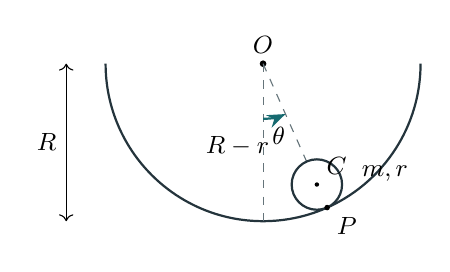
\begin{tikzpicture}[font=\small]
\draw[object](-2,0)arc(180:360:2);\fill(0,0)circle(1.2pt)node[above]{$O$};
\draw[guide](0,0)--(.813473286,-1.827090915);\draw[guide](0,0)--(0,-2);
\draw[object,fill=white](.683317561,-1.534756369)circle(.32);
\fill(.683317561,-1.534756369)circle(.8pt)node[above right]{$C$};
\fill(.813473286,-1.827090915)circle(1pt)node[below right]{$P$};
\draw[motion](0,-.7)arc(-90:-66:.7);\node at(.2,-.92){$\theta$};
\draw[<->](-2.5,0)--(-2.5,-2)node[midway,left]{$R$};
\node[left]at(.2,-1.05){$R-r$};\node[right]at(1.13,-1.4){$m,r$};
\end{tikzpicture}\figcaption{图 7.12}\end{minipage}\end{center}

\workarea

\clearpage

\pdfbookmark[2]{第 13 题 物体在两薄壁圆筒上纯滚的振动}{q13}

\section*{第 13 题\quad 物体在两薄壁圆筒上纯滚的振动}

\tagline{M-07-13}

如图7.13,质量为\(M\)的物体放置在两个完全相同的质量均为\(m\)的薄壁中空圆筒上.物体两侧系着两个完全相同的劲度系数均为\(k\)的弹簧,两弹簧的另一端固定,开始时两弹簧均为原长.设物体在两薄圆筒上作纯滚动.试求振动圆频率.
两筒与地面、上方物体接触处均不滑动；上方物体不转动，两处接触保持。

\begin{center}\begin{minipage}{\linewidth}\centering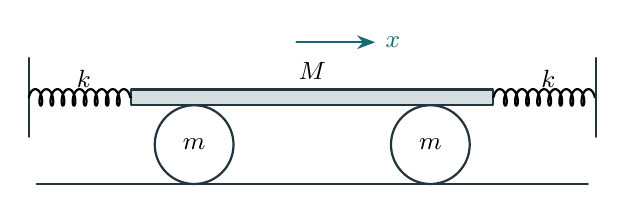
\begin{tikzpicture}[line cap=round,line join=round,spring/.style={decorate,decoration={coil,aspect=.45,segment length=4pt,amplitude=3pt},thick}]\draw[object] (-2,-.5)--(5,-.5);\draw[object] (0,0) circle (.5);\draw[object] (3,0) circle (.5);\draw[object,fill=rulegray] (-.8,.5) rectangle (3.8,.7);\node[above] at (1.5,.7) {$M$};\draw[object](-2.1,.1)--(-2.1,1.1);\draw[spring](-2.1,.6)--(-.8,.6);\draw[spring](3.8,.6)--(5.1,.6);\draw[object](5.1,.1)--(5.1,1.1);\node[above] at (-1.4,.6) {$k$};\node[above] at (4.5,.6) {$k$};\node at (0,0) {$m$};\node at (3,0) {$m$};\draw[motion] (1.3,1.3)--(2.3,1.3) node[right] {$x$};\end{tikzpicture}\figcaption{图 7.13}\end{minipage}\end{center}

\workarea

\clearpage

\pdfbookmark[2]{第 14 题 旋转圆盘导轨中弹簧小球的振动}{q14}

\section*{第 14 题\quad 旋转圆盘导轨中弹簧小球的振动}

\tagline{M-07-14}

如图,圆盘绕通过中心O点的竖直轴在水平面内匀速转动,角速度为\(\omega\),质量为\(m\)的小球被约束在圆盘上的光滑导轨AB内运动.小球与劲度系数为\(k\)的弹簧相连(\(k>m\omega^{2}\)),弹簧另一端固定在圆盘A点.弹簧为原长时,小球位于\(P\)点,\(OP=r_{0}\),且\(OP\perp AB\),将小球从\(P\)点沿导轨拉开距离\(a\)后从静止释放.在圆盘参考系中考察小球的运动.

试求小球的平衡位置. 2. 试证明小球作简谐振动, 并求圆频率. 3.
试求导轨施于小球的水平力随时间的变化规律. 4. 试问当 \(k<m \omega^{2}\)
时小球怎样运动.

\begin{center}\begin{minipage}{\linewidth}\centering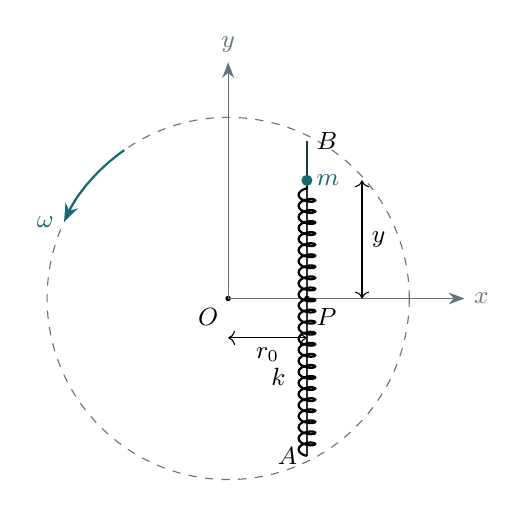
\begin{tikzpicture}[font=\small,spring/.style={decorate,decoration={coil,aspect=.45,segment length=4pt,amplitude=3pt},thick}]
\draw[guide](0,0)circle(2.3);\fill(0,0)circle(1pt)node[below left]{$O$};
\draw[axis](0,0)--(3,0)node[right]{$x$};\draw[axis](0,0)--(0,3)node[above]{$y$};
\draw[object](1,-2)--(1,2);\draw[spring](1,-2)--(1,1.5);
\node[left]at(1,-2){$A$};\fill(1,0)circle(1pt)node[below right]{$P$};\node[right]at(1,2){$B$};
\fill[accent](1,1.5)circle(2pt)node[right]{$m$};\node[left]at(.85,-1){$k$};
\draw[<->](0,-.5)--(1,-.5)node[midway,below]{$r_0$};
\draw[<->](1.7,0)--(1.7,1.5)node[midway,right]{$y$};
\draw[motion](-1.319225804,1.884049702)arc(125:155:2.3)node[left]{$\omega$};
\end{tikzpicture}\figcaption{图 7.14}\end{minipage}\end{center}

\workarea

\clearpage

\pdfbookmark[2]{第 15 题 圆周弹簧质点受径向轻击后的径向频率}{q15}

\section*{第 15 题\quad 圆周弹簧质点受径向轻击后的径向频率}

\tagline{M-07-15}

如图,质量为\(m\)的小球在光滑水平桌面上以角速度\(\omega\)作匀速圆周运动.所需的向心力由与小球相连的弹簧提供,弹簧的劲度系数为\(k\),另一端固定.今沿径向轻击小球.试求小球径向振动的频率.

\begin{center}\begin{minipage}{\linewidth}\centering\begin{tikzpicture}[font=\small,spring/.style={decorate,decoration={coil,aspect=.45,segment length=4pt,amplitude=3pt},thick}]
\draw[guide](0,0)circle(2);\fill(0,0)circle(1.2pt)node[below left]{$O$};
\draw[spring](0,0)--(2,0);\fill[accent](2,0)circle(2pt)node[below right]{$m$};
\draw[motion](2,0)--(2,.85)node[right]{$R\omega$};
\draw[force](2,0)--(2.9,0)node[right]{$J_r$（径向）};
\draw[<->](0,-.65)--(1.2,-.65)node[midway,below]{$r_0$};
\draw[<->](0,-1.25)--(2,-1.25)node[midway,below]{$R$};
\end{tikzpicture}\figcaption{图 7.15}\end{minipage}\end{center}

\workarea

\clearpage

\pdfbookmark[2]{第 16 题 有限振幅单摆周期的二级近似}{q16}

\section*{第 16 题\quad 有限振幅单摆周期的二级近似}

\tagline{M-07-16}

计算单摆周期时,若摆幅 \(\theta_{0}\) 较小,可采用一级近似
\(\sin \theta \approx \theta\),算出的周期为
\(T_{0}=2 \pi \sqrt{\frac{l}{g}}\),其中 \(l\) 为摆长.若 \(\theta_{0}\)
不算小,就应取二级近似.试导出单摆周期 \(T\) 与摆幅 \(\theta_{0}\) 的关系.

\begin{center}\begin{minipage}{\linewidth}\centering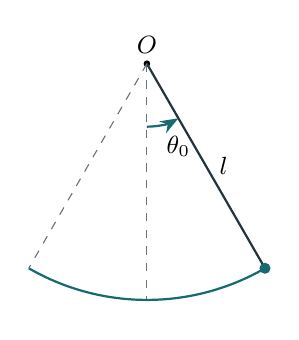
\begin{tikzpicture}[font=\small]
\fill(0,0)circle(1.2pt)node[above]{$O$};
\draw[object](0,0)--(1.5,-2.598076211);\fill[accent](1.5,-2.598076211)circle(2pt);
\draw[guide](0,0)--(0,-3);\draw[guide](0,0)--(-1.5,-2.598076211);
\draw[traj](-1.5,-2.598076211)arc(-120:-60:3);
\draw[motion](0,-.8)arc(-90:-60:.8);\node at(.4,-1.05){$\theta_0$};
\node[right]at(.8,-1.3){$l$};
\end{tikzpicture}\figcaption{图 7.16}\end{minipage}\end{center}

\workarea

\clearpage

\pdfbookmark[2]{第 17 题 谐振子的相积分与能量频率关系}{q17}

\section*{第 17 题\quad 谐振子的相积分与能量频率关系}

\tagline{M-07-17}

对于谐振子,若广义动量为\(p\),广义坐标为\(q\),则有\(\oint p\mathrm{d}q=\frac{E}{\nu}\),其中\(E\)为谐振子的能量,\(\nu\)为振动频率.积分在振动的一个周期内进行.试就弹簧振子和单摆的情况证明此式.

\begin{center}\begin{minipage}{\linewidth}\centering\begin{tikzpicture}[line cap=round,line join=round,spring/.style={decorate,decoration={coil,aspect=.45,segment length=4pt,amplitude=3pt},thick}]\draw[axis] (-2.4,0)--(2.5,0) node[right] {$x$};\draw[axis] (0,-1.7)--(0,1.8) node[above] {$p_x$};\draw[traj] (0,0) ellipse (2 and 1.3);\node at (0,-2.1) {弹簧振子};\begin{scope}[xshift=6cm]\draw[axis] (-2.4,0)--(2.5,0) node[right] {$\theta$};\draw[axis] (0,-1.7)--(0,1.8) node[above] {$p_\theta$};\draw[traj] (0,0) ellipse (2 and 1.3);\node at (0,-2.1) {小角单摆};\end{scope}\end{tikzpicture}\figcaption{图 7.17}\end{minipage}\end{center}

\workarea

\clearpage

\pdfbookmark[2]{第 18 题 T形导轨约束细杆的小振动与碰撞}{q18}

\section*{第 18 题\quad T形导轨约束细杆的小振动与碰撞}

\tagline{M-07-18}

如图7.18,T形导轨固定在铅垂面内,质量为\(m\)、全长为\(l\)的刚性均匀细杆两端约束在T形导轨中,可沿导轨作无摩擦的滑动.1.试求细杆作小振幅摆动时的振动周期.2.当细杆摆至右方适当角度刚好达到静止时(如图7.18中虚线所示),一质量也为\(m\)的小球以速度\(v_{0}\)沿水平方向经导轨与细杆上端相碰.设碰撞无机械能损失,碰后小球速度变为零,细杆则回摆到左方与水平导轨平行时刚好静止.试问\(v_{0}\)应为多大?

\begin{center}\begin{minipage}{\linewidth}\centering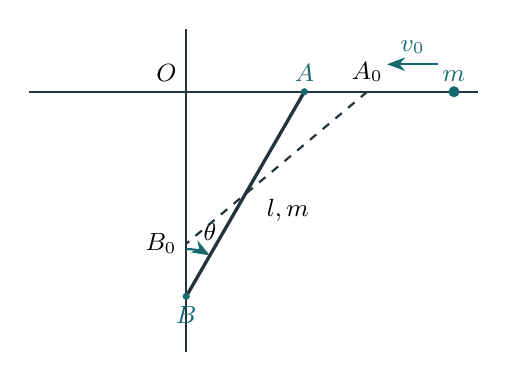
\begin{tikzpicture}[font=\small]
\draw[object](-2,0)--(3.7,0);\draw[object](0,.8)--(0,-3.3);
\draw[object,very thick](1.5,0)--(0,-2.598076211);
\fill[accent](1.5,0)circle(1.3pt)node[above]{$A$};
\fill[accent](0,-2.598076211)circle(1.3pt)node[below]{$B$};
\node[above left]at(0,0){$O$};\node[right]at(.9,-1.5){$l,m$};
\draw[motion](0,-1.998076211)arc(90:60:.6);\node at(.3,-1.78){$\theta$};

\draw[object,dashed](2.298133329,0)--(0,-1.928362829);
\node[above]at(2.298133329,0){$A_0$};\node[left]at(0,-1.928362829){$B_0$};
\fill[accent](3.4,0)circle(2pt)node[above]{$m$};\draw[motion](3.2,.35)--(2.55,.35)node[midway,above]{$v_0$};
\end{tikzpicture}\figcaption{图 7.18}\end{minipage}\end{center}

\workarea

\clearpage

\pdfbookmark[2]{第 19 题 两质量弹簧系统的相对振动}{q19}

\section*{第 19 题\quad 两质量弹簧系统的相对振动}

\tagline{M-07-19}

如图,在光滑水平面上,质量为\(m_{1}\)和\(m_{2}\)的两物体用劲度系数为\(k\)的弹簧相连.当弹簧为原长时,\(m_{1}\)与\(m_{2}\)相距\(l_{0}\),把弹簧压缩距离\(a\)后从静止释放.试求\(m_{1}\)和\(m_{2}\)的振动表达式.

\begin{center}\begin{minipage}{\linewidth}\centering\begin{tikzpicture}[font=\small,spring/.style={decorate,decoration={coil,aspect=.45,segment length=4pt,amplitude=3pt},thick}]
\draw[object,fill=white](-2.55,-.25)rectangle(-1.95,.25);\node at(-2.25,0){$m_1$};
\draw[object,fill=white](.45,-.25)rectangle(1.05,.25);\node at(.75,0){$m_2$};
\draw[spring](-1.95,0)--(.45,0);\node[above]at(-.75,.3){$k,l_0$};
\draw[guide](-3.5,-.3)--(1.6,-.3);\draw[guide](0,.25)--(0,.85);\node[above]at(0,.85){$C$};
\draw[<->](-2.25,-.65)--(.75,-.65)node[midway,below]{$l_0-a$};
\draw[axis](-3.5,-1.3)--(1.6,-1.3)node[right]{$x$};\node[below]at(0,-1.3){$0$};
\node at(-.6,-1.95){初始压缩状态，图示位置取$m_2=3m_1$};
\end{tikzpicture}\figcaption{图 7.19}\end{minipage}\end{center}

\workarea

\clearpage

\pdfbookmark[2]{第 20 题 缓慢缩短摆长时的振幅变化}{q20}

\section*{第 20 题\quad 缓慢缩短摆长时的振幅变化}

\tagline{M-07-20}

如图,单摆的原长为\(l_{0}\),在摆动过程中缓慢上拉,悬点位置不变而摆长逐渐缩短.试求当摆长缩短为原长之半,即\(l=\frac{l_{0}}{2}\)时的振幅与原振幅之比.

采用小角、缓慢变化的近似；分别说明角振幅与弧长振幅的变化。

\begin{center}\begin{minipage}{\linewidth}\centering\begin{tikzpicture}[font=\small]
\fill(0,0)circle(1.2pt)node[above]{$O$};\draw[object](0,0)--(1.026060430,-2.819077862);
\fill[accent](1.026060430,-2.819077862)circle(2pt);\draw[guide](0,0)--(0,-3.2);
\draw[guide](0,0)--(-1.026060430,-2.819077862);
\draw[motion](.7,-1.923234838)--(.35,-.961617419);\node[right]at(1.25,-1.1){缓慢上拉};
\draw[motion](0,-.75)arc(-90:-70:.75);\node at(.2,-1.0){$\theta$};
\node[right]at(.8,-2){$l$};
\end{tikzpicture}\figcaption{图 7.20\quad $l$为当前摆长，$\theta$为瞬时摆角；箭头表示缓慢上拉。}\end{minipage}\end{center}

\workarea

\clearpage

\pdfbookmark[2]{第 21 题 小虫沿刚性摆杆爬行时的频率与振幅}{q21}

\section*{第 21 题\quad 小虫沿刚性摆杆爬行时的频率与振幅}

\tagline{M-07-21}

如图,质量为\(M\)、长为\(L\)的均匀刚性细杆的一端悬挂,可在铅垂面内绕悬点无摩擦地

摆动．质量为 \(m=\frac{M}{3}\) 的小虫相对杆以速度 \(v_{\mathrm{L}}\)
缓慢地沿杆向下爬行．开始时,杆静止并与竖直线夹 \(\theta_{0}\) 角(设
\(\theta_{0}\)
很小)；小虫位于杆上端的悬点．放开后,杆开始摆动,小虫开始爬行．

试求:1. 小虫沿杆爬行 \(l\) 距离时,杆摆动的圆频率.2.
小虫爬到杆下端时,杆摆动的幅度.

\begin{center}\begin{minipage}{\linewidth}\centering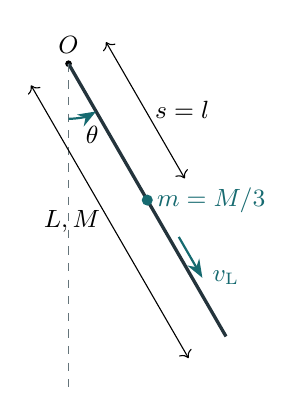
\begin{tikzpicture}[font=\small]
\fill(0,0)circle(1.2pt)node[above]{$O$};\draw[object,very thick](0,0)--(2,-3.464101615);
\fill[accent](1,-1.732050808)circle(2pt)node[right]{$m=M/3$};\draw[guide](0,0)--(0,-4.1);
\draw[<->](-.476313972,-.275)--(1.523686028,-3.739101615)node[midway,left]{$L,M$};
\draw[<->](.476313972,.275)--(1.476313972,-1.457050808)node[midway,right]{$s=l$};
\draw[motion](1.4,-2.2)--(1.7,-2.719615242)node[right]{$v_{\rm L}$};
\draw[motion](0,-.7)arc(-90:-60:.7);\node at(.3,-.9){$\theta$};
\end{tikzpicture}\figcaption{图 7.21}\end{minipage}\end{center}

\workarea

\clearpage

\pdfbookmark[2]{第 22 题 旋转圆盘支架上摆球的平衡与小振动}{q22}

\section*{第 22 题\quad 旋转圆盘支架上摆球的平衡与小振动}

\tagline{M-07-22}

如图7.22,圆盘在水平面内以匀角速\(\Omega\)绕竖直轴OO'旋转,盘上固连着两根同样高度的竖直支架.质量为\(m\)的小球与质量可忽略不计的\(T\)字形细杆相连,水平杆由支架支承,与小球相连的杆长为\(l\),悬点\(O'\)在转轴上,整个系统可在支架上无摩擦地摆动.

试求:1. 小球的平衡位置 .2. 小球作小幅摆动时的圆频率.

\begin{center}\begin{minipage}{\linewidth}\centering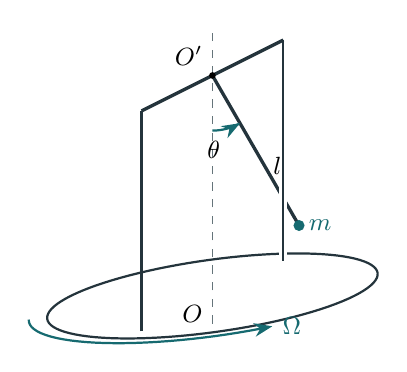
\begin{tikzpicture}[font=\small,x={(1cm,0cm)},y={(.6cm,.3cm)},z={(0cm,1cm)}]
\draw[object,variable=\u,domain=0:360,samples=101]plot({1.8*cos(\u)},{1.8*sin(\u)},0);
\draw[object](0,-1.5,0)--(0,-1.5,2.8);\draw[guide](0,0,-.35)--(0,0,3.4);
\draw[object,very thick](0,0,2.8)--(1.1,0,.894744112);\fill[accent](1.1,0,.894744112)circle(2pt)node[right]{$m$};
\draw[white,line width=3pt](0,1.5,0)--(0,1.5,2.8);\draw[object](0,1.5,0)--(0,1.5,2.8);
\draw[object,very thick](0,-1.5,2.8)--(0,1.5,2.8);
\fill(0,0,2.8)circle(1.2pt)node[above left]{$O'$};\node[below left]at(0,0,0){$O$};
\draw[motion,variable=\u,domain=0:30,samples=31]plot({.7*sin(\u)},0,{2.8-.7*cos(\u)});
\node[left]at(.22,0,1.85){$\theta$};\node[right]at(.65,0,1.65){$l$};
\draw[motion,variable=\u,domain=210:320,samples=31]plot({2*cos(\u)},{2*sin(\u)},0)node[right]{$\Omega$};
\end{tikzpicture}\figcaption{图 7.22}\end{minipage}\end{center}

\workarea

\clearpage

\pdfbookmark[2]{第 23 题 弹性碰撞激发弹簧连接双质点振动}{q23}

\section*{第 23 题\quad 弹性碰撞激发弹簧连接双质点振动}

\tagline{M-07-23}

如图,在光滑水平面上有三质点A、B、C,质量分别为\(m_{1}\)、\(m_{2}\)和\(m_{3}\),三质点位于同一直线上,开始时B和C静止,用劲度系数为k的弹簧(质量忽略)相连.开始时弹簧无形变。质点A以初速\(v_{0}\)沿连线方向与B作完全弹性碰撞.

以 \(A\) 和 \(B\) 的碰撞点为坐标原点, 连线为 \(x\) 轴, 试求碰后质点
\(B\) 的运动规律. 2. 设 \(m_{2}=m_{3}=m\), 为使质点 \(A\) 和 \(B\)
在碰后重新相遇, 但不相碰(即相遇时速度相同), 试问比值 \(\frac{m_{1}}{m}\)
应为多少?

\begin{center}\begin{minipage}{\linewidth}\centering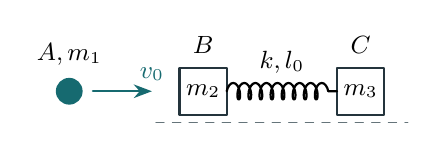
\begin{tikzpicture}[line cap=round,line join=round,spring/.style={decorate,decoration={coil,aspect=.45,segment length=4pt,amplitude=3pt},thick}]\fill[accent] (-1.7,0) circle (.17);\node[above] at (-1.7,.2) {$A,m_1$};\draw[motion] (-1.4,0)--(-.65,0) node[above] {$v_0$};\draw[object,fill=white] (-0.3,-.3) rectangle (0.3,.3);\node at (0,0) {$m_2$};\draw[object,fill=white] (1.7,-.3) rectangle (2.3,.3);\node at (2,0) {$m_3$};\draw[spring] (0.30000000000000004,0)--(1.7,0);\draw[guide] (-.6,-.4)--(2.6,-.4);\node[above] at (0,.35) {$B$};\node[above] at (2,.35) {$C$};\node[above] at (1,.1) {$k,l_0$};\end{tikzpicture}\figcaption{图 7.23}\end{minipage}\end{center}

\workarea

\clearpage

\pdfbookmark[2]{第 24 题 三球双弹簧系统的特征频率和振型}{q24}

\section*{第 24 题\quad 三球双弹簧系统的特征频率和振型}

\tagline{M-07-24}

如图7.24,质量为\(M\)的小球两侧分别用劲度系数均为\(k\)的弹簧与两个质量均为\(m\)的小球连成一直线,水平放置,忽略一切阻力和摩擦力.试求特征频率和振动模式.

\begin{center}\begin{minipage}{\linewidth}\centering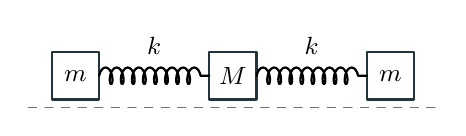
\begin{tikzpicture}[line cap=round,line join=round,spring/.style={decorate,decoration={coil,aspect=.45,segment length=4pt,amplitude=3pt},thick}]\draw[object,fill=white] (-0.3,-.3) rectangle (0.3,.3);\node at (0,0) {$m$};\draw[object,fill=white] (1.7,-.3) rectangle (2.3,.3);\node at (2,0) {$M$};\draw[spring] (0.30000000000000004,0)--(1.7,0);\draw[object,fill=white] (3.7,-.3) rectangle (4.3,.3);\node at (4,0) {$m$};\draw[spring] (2.3,0)--(3.7,0);\draw[guide] (-.6,-.4)--(4.6,-.4);\node[above] at (1,.15) {$k$};\node[above] at (3,.15) {$k$};\end{tikzpicture}\figcaption{图 7.24}\end{minipage}\end{center}

\workarea

\clearpage

\pdfbookmark[2]{第 25 题 两端弹簧支承木板的小振动特征频率}{q25}

\section*{第 25 题\quad 两端弹簧支承木板的小振动特征频率}

\tagline{M-07-25}

如图,质量为 \(m\) 、长为 \(l\) 的均匀长方形木板由劲度系数分别为
\(k_{1}\) 和 \(k_{2}\)
的两竖直弹簧在两端支撑,平衡时木板位于水平面.试求木板作小幅振动时的特征频率.

\begin{center}\begin{minipage}{\linewidth}\centering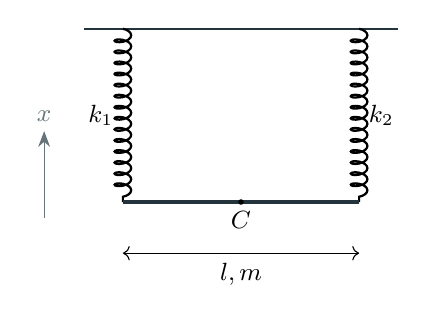
\begin{tikzpicture}[font=\small,spring/.style={decorate,decoration={coil,aspect=.45,segment length=4pt,amplitude=3pt},thick}]
\draw[object](-2,2.2)--(2,2.2);\draw[spring](-1.5,2.2)--(-1.5,0);\draw[spring](1.5,2.2)--(1.5,0);
\draw[object,very thick](-1.5,0)--(1.5,0);\fill(0,0)circle(1pt)node[below]{$C$};
\node[left]at(-1.5,1.1){$k_1$};\node[right]at(1.5,1.1){$k_2$};
\draw[<->](-1.5,-.65)--(1.5,-.65)node[midway,below]{$l,m$};
\draw[axis](-2.5,-.2)--(-2.5,.9)node[above]{$x$};
\end{tikzpicture}\figcaption{图 7.25}\end{minipage}\end{center}

\workarea

\clearpage

\pdfbookmark[2]{第 26 题 两个弹簧耦合单摆的简正模式}{q26}

\section*{第 26 题\quad 两个弹簧耦合单摆的简正模式}

\tagline{M-07-26}

如图7.26,两个完全相同的单摆并排悬挂,摆球质量均为\(m\),摆长均为\(l\),两摆球用劲度系数为\(k\)的轻质弹簧连接,弹簧原长等于两悬点之间的距离.忽略空气阻力.上述振

动系统称为耦合摆．在小角摆动的条件下，1.
试求耦合摆的特征频率，并写出两摆球运动方程的一般表达式. 2.
试讨论耦合摆在不同初始条件下的几种典型运动情况．

\begin{center}\begin{minipage}{\linewidth}\centering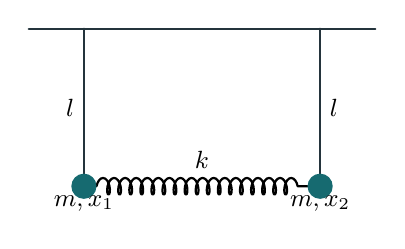
\begin{tikzpicture}[line cap=round,line join=round,spring/.style={decorate,decoration={coil,aspect=.45,segment length=4pt,amplitude=3pt},thick}]\draw[object] (-.7,2)--(3.7,2);\draw[object] (0,2)--(0,0);\draw[object] (3,2)--(3,0);\draw[spring] (.16,0)--(2.84,0);\fill[accent] (0,0) circle (.16);\fill[accent] (3,0) circle (.16);\node[below] at (0,0) {$m,x_1$};\node[below] at (3,0) {$m,x_2$};\node[above] at (1.5,.1) {$k$};\node[left] at (0,1) {$l$};\node[right] at (3,1) {$l$};\end{tikzpicture}\figcaption{图 7.26}\end{minipage}\end{center}

\workarea

\clearpage

\pdfbookmark[2]{第 27 题 六球环形弹簧链的特征频率}{q27}

\section*{第 27 题\quad 六球环形弹簧链的特征频率}

\tagline{M-07-27}

如图,6个质量均为\(m\)的小球串在光滑圆环上,彼此间用劲度系数均为\(k\)的6个弹簧相连,整个系统在水平面内.当各小球处在平衡位置时,弹簧均为原长.试求特征频率.

沿环的切向弧长量取位移；弹簧按沿环导向的模型处理，伸长增量为相邻位移之差。

\begin{center}\begin{minipage}{\linewidth}\centering\begin{tikzpicture}[font=\small,line cap=round,spring/.style={decorate,decoration={coil,aspect=.45,segment length=4pt,amplitude=2.5pt},thick,accent}]
\draw[guide](0,0)circle(2);
\foreach \j in {0,...,5}{\pgfmathsetmacro{\aa}{60*\j}\pgfmathsetmacro{\bb}{60*(\j+1)}\draw[spring](\aa:2)arc[start angle=\aa,end angle=\bb,radius=2];}
\foreach \j in {0,...,5}{\pgfmathsetmacro{\aa}{60*\j}\pgfmathtruncatemacro{\nn}{\j+1}\fill[accent](\aa:2)circle(.13);\node at(\aa:2.5){$\nn$};}
\node at(0,.25){沿环导向};\node at(0,-.25){$m,\ k$};
\draw[motion](15:2.85)arc[start angle=15,end angle=45,radius=2.85]node[above right]{位移正向};
\end{tikzpicture}\figcaption{图 7.27}\end{minipage}\end{center}

\workarea

\clearpage

\pdfbookmark[2]{第 28 题 圆周弹簧质点链的简正模式与频带}{q28}

\section*{第 28 题\quad 圆周弹簧质点链的简正模式与频带}

\tagline{M-07-28}

三个质量各为\(m\)的质点由未伸长的无质量弹簧连接在一起达到平衡．每个弹簧的劲度系数为\(k\)，它们被限制在圆周上运动，如图7.28所示．

若每一质点 \(m\) 分别有偏离平衡位置的小位移 \(u_{1}, u_{2}\) 和
\(u_{3}\), 试写出每一质点的运动方程

试验证此系统有下列简谐式解

\[
u_{ n } = a_{ n } \cos \omega t
\]

其加速度为\(-\omega^{2}u_{n}\),此处\(a_{n}(n=1,2,3)\)是恒振幅,角频率\(\omega\)有下列三个可能的取值,即

\[
\sqrt{ 3 } \omega_{ 0 } , \sqrt{ 3 } \omega_{ 0 } , 0
\]

其中\(\omega_{0}^{2}=\frac{k}{m}\).

将这由弹簧与质点交替连接的系统扩充到 \(N\) 个质点, 每一质点 \(m\)
由弹簧与相邻质点连接. 起初弹簧未伸长, 处于平衡, 当质点偏离平衡时, 用第
\(n\) 个质点的位移和相邻质点的位移表示出第 \(n\) 个质点
\((n=1,2, \cdots, N)\) 的运动方程. 试验证

\[
u_{ n } ( t ) = a_{ s } \sin \left( \frac{ 2 n s \pi } { N } + \phi \right) \cos \omega_{ s } t
\]

是振荡解,式中 \(s=1,2,\cdots,N,n=1,2,\cdots,N,\varphi\)
为一任意相位,角频率 \(\omega\), 由下式给出

\[
\omega_{ s } = 2 \omega_{ 0 } \sin \bigg ( \frac{ s \pi } { N } \bigg )
\]

而 \(a_{s}(s=1,2,\cdots,N)\) 是与 \(n\) 无关的恒振幅.

试叙述对于一个含有无穷多个质点的链条,频率的可能范围.

试确定\(\frac{u_{n}}{u_{n+1}}\)的比值.

当 \(N\) 很大时,对于下列 \((a),(b)\) 两种情况,试画出说明时刻 \(t\)
质点的位移与该质点在链上编号之间关系的草图.

(a)低频解.

\((b)\omega_{\mathrm{s}}=\omega_{\mathrm{max}}\) ,其中
\(\omega_{\mathrm{max}}\) 是最大的频率解 .

5.若质点之一用质量 \(m^{\prime} \ll m\)
的质点代替,试估计角频率分布将发生怎样的主要变化.

试在上面结果的基础上定性地描述,由质量为 \(m\) 和 \(m'\)
交替联接的双原子链会有怎样形式的频谱.

提示：

\[
\begin{array}{r} { \sin ( A + B ) = \sin A \, \cos B + \cos A \, \sin B } \\{ \sin A + \sin B = 2 \sin \frac{ A + B } { 2 } \, \cos \frac{ A - B } { 2 } } \\{ 2 \sin^{2} A = 1 - \cos 2 A } \end{array}
\]

沿环的切向弧长量取位移；弹簧按沿环导向的模型处理，伸长增量为相邻位移之差。

\begin{center}\begin{minipage}{\linewidth}\centering\begin{tikzpicture}[font=\small,line cap=round,spring/.style={decorate,decoration={coil,aspect=.45,segment length=4pt,amplitude=2pt},thick,accent}]
\foreach \sh/\NN/\tit in {0/3/三质点,6/10/$N$质点示例}{
\begin{scope}[xshift=\sh cm]
\draw[guide](0,0)circle(1.45);
\pgfmathtruncatemacro{\last}{\NN-1}
\foreach \j in {0,...,\last}{\pgfmathsetmacro{\aa}{360*\j/\NN}\pgfmathsetmacro{\bb}{360*(\j+1)/\NN}\draw[spring](\aa:1.45)arc[start angle=\aa,end angle=\bb,radius=1.45];}
\foreach \j in {0,...,\last}{\pgfmathsetmacro{\aa}{360*\j/\NN}\pgfmathtruncatemacro{\nn}{\j+1}\fill[accent](\aa:1.45)circle(.10);\node at(\aa:1.84){$\nn$};}
\node at(0,0){\tit};\node at(0,-2.25){沿环导向，位移按逆时针为正};
\end{scope}}
\end{tikzpicture}\figcaption{图 7.28}\end{minipage}\end{center}

\par\vspace{5mm}\noindent{\small\color{muted}作答区}\par\vspace{4mm}\noindent\textcolor{rulegray}{\rule{\linewidth}{0.3pt}}\par\vspace{16mm}\noindent\textcolor{rulegray}{\rule{\linewidth}{0.3pt}}\par\vspace{16mm}\noindent\textcolor{rulegray}{\rule{\linewidth}{0.3pt}}

\clearpage

\pdfbookmark[2]{第 29 题 带阻尼器摆的等效阻尼振动}{q29}

\section*{第 29 题\quad 带阻尼器摆的等效阻尼振动}

\tagline{M-07-29}

如图,细杆长 \(l\),上端 \(O\) 悬挂,下端与质量为 \(m\) 的摆球相连,摆球可绕
\(O\) 轴无摩擦地摆动. 今在细杆的 \(A\) 点经连杆接一阻尼器,阻尼力 \(f\)
沿水平方向,其大小

与阻尼板的速度 \(v\) 成正比,即 \(f=\gamma v\), \(\gamma\) 为阻力系数. 设
\(OA=a\), 细杆、连杆、阻尼板等的质量均远小于 \(m\), 可忽略不计,
阻尼较弱. 试求小幅阻尼振动的对数减缩, 以及一周期内损失能量的百分比.

\begin{center}\begin{minipage}{\linewidth}\centering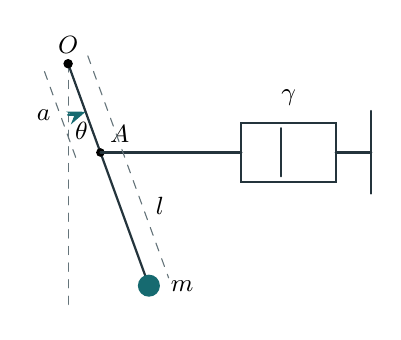
\begin{tikzpicture}[font=\small,line cap=round]
\coordinate(O)at(0,0);\coordinate(A)at(.410424172,-1.127631145);\coordinate(B)at(1.026060430,-2.819077862);
\draw[guide](0,0)--(0,-3.15);\draw[object](O)--(B);\fill(O)circle(.06);\node[above]at(O){$O$};
\fill[accent](B)circle(.14);\node[right]at(1.18,-2.82){$m$};\fill(A)circle(.055);\node[above right]at(A){$A$};
\draw[object](A)--(2.2,-1.127631145);\draw[object](2.2,-1.5)rectangle(3.4,-.75);
\draw[object](2.7,-1.43)--(2.7,-.82);\draw[object](3.4,-1.127631145)--(3.85,-1.127631145);
\draw[object](3.85,-1.65)--(3.85,-.6);\node[above]at(2.8,-.65){$\gamma$};
\draw[motion](-90:.65)arc[start angle=-90,end angle=-70,radius=.65];\node at(.17,-.85){$\theta$};
\draw[guide](-.3,-.1)--(.110424172,-1.227631145);\node[left]at(-.1,-.65){$a$};
\draw[guide](.25,.1)--(1.276060430,-2.719077862);\node[right]at(.99,-1.8){$l$};

\end{tikzpicture}\figcaption{图 7.29}\end{minipage}\end{center}

\workarea

\clearpage

\pdfbookmark[2]{第 30 题 临界阻尼是否最快回到平衡位置}{q30}

\section*{第 30 题\quad 临界阻尼是否最快回到平衡位置}

\tagline{M-07-30}

质量为\(m\)的质点在弹性力和阻尼力的作用下沿\(x\)轴运动．取平衡位置为坐标原点，弹性力为\(-kx\)，阻尼力为\(-\gamma\dot{x}\)．试问，是否在临界阻尼情况下，质点回到平衡位置一定最快？

\begin{center}\begin{minipage}{\linewidth}\centering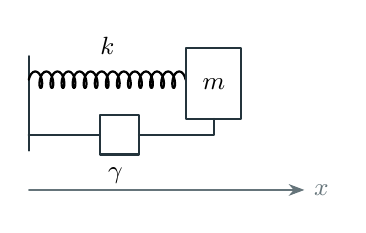
\begin{tikzpicture}[line cap=round,line join=round,spring/.style={decorate,decoration={coil,aspect=.45,segment length=4pt,amplitude=3pt},thick}]\draw[object] (0,-.6)--(0,.6);\draw[spring] (0,.3)--(2,.3);\draw[object,fill=white] (2,-.2) rectangle (2.7,.7);\node at (2.35,.25) {$m$};\draw[object] (0,-.4)--(.9,-.4);\draw[object] (.9,-.65) rectangle (1.4,-.15);\draw[object] (1.4,-.4)--(2.35,-.4)--(2.35,-.2);\node[below] at (1.1,-.7) {$\gamma$};\draw[axis] (0,-1.1)--(3.5,-1.1) node[right] {$x$};\node[above] at (1,.5) {$k$};\end{tikzpicture}\figcaption{图 7.30}\end{minipage}\end{center}

\workarea

\clearpage

\pdfbookmark[2]{第 31 题 容器振动驱动下的阻尼受迫振子}{q31}

\section*{第 31 题\quad 容器振动驱动下的阻尼受迫振子}

\tagline{M-07-31}

如图7.31,充满液体的容器在竖直方向上下振动,质量为\(m\)的重物由劲度系数为\(k\)的弹簧悬挂,浸没在液体之中.设悬点随容器振动的规律为\(x_{H}=A\cos\omega t\),设液体的阻尼系数为\(\gamma\)(弱阻尼),并假定液体的浮力恒定.

若 \(\omega=\omega_{0}\), 试求稳定后重物的振动表达式, 其中
\(\omega_{0}=\sqrt{\frac{k}{m}}\) 为弹簧振子的固有圆频率.

若 \(\omega \gg \omega_{0}\), 试求稳定后重物的振动表达式.

若 \(\omega \gg \omega_{0}\), 且当容器达到最高点时突然停止不动,
试求此后重物的振动表达式.

试画出容器突然停止以前和以后的振动曲线.

\begin{center}\begin{minipage}{\linewidth}\centering\begin{tikzpicture}[font=\small,line cap=round,spring/.style={decorate,decoration={coil,aspect=.45,segment length=4pt,amplitude=3pt},thick}]
\fill[rulegray](-1.1,-1.9)rectangle(1.1,1.85);
\draw[object](-1.2,2.2)--(-1.2,-2)--(1.2,-2)--(1.2,2.2);\draw[object](-1.2,2)--(1.2,2);
\draw[spring](.3,2)--(.3,-.2);\draw[object,fill=white](-.1,-.8)rectangle(.7,-.2);\node at(.3,-.5){$m$};\node[right]at(.5,.8){$k$};
\draw[guide](-1.5,1.4)--(1.7,1.4);\node[right]at(1.7,1.4){$H_0$};
\draw[guide](-1.5,-.9)--(2.5,-.9);\node[right]at(2.5,-.9){$O:\ x=0$};
\draw[motion](-1.7,1.4)--(-1.7,2)node[midway,left]{$x_H$};
\draw[motion](1.6,-.9)--(1.6,-.5)node[midway,right]{$x$};
\draw[axis](2.7,-.5)--(2.7,1.1)node[above]{向上};\node at(.1,-1.55){液体随容器平动};

\end{tikzpicture}\figcaption{图 7.31}\end{minipage}\end{center}

\workarea

\clearpage

\pdfbookmark[2]{第 32 题 受周期外力三滑块弹簧链的响应}{q32}

\section*{第 32 题\quad 受周期外力三滑块弹簧链的响应}

\tagline{M-07-32}

如图,质量均为\(m\)的三个滑块放置在光滑水平桌面上,彼此以原长为\(x_{0}\)、劲度系数为

k 的二个相同弹簧连接起来. 开始时三滑块静止, 滑块 A 位于原点 O,
两弹簧均为原长. 对滑块 A 施以周期性外力 F, 已知
\(F=F_{0} \cos \omega t\), 在水平方向并沿三滑块连线.
试求振动系统的特征频率, 并写出滑块 C 的运动方程.

\begin{center}\begin{minipage}{\linewidth}\centering\begin{tikzpicture}[font=\small,line cap=round,spring/.style={decorate,decoration={coil,aspect=.45,segment length=4pt,amplitude=3pt},thick}]
\draw[spring](.3,0)--(1.7,0);\draw[spring](2.3,0)--(3.7,0);
\foreach \xx/\name in {0/A,2/B,4/C}{\draw[object,fill=white](\xx-.3,-.3)rectangle(\xx+.3,.3);\node at(\xx,0){$m$};\node[above]at(\xx,.4){$\name$};}
\draw[guide](-.6,-.4)--(4.8,-.4);\draw[force](-1.6,0)--(-.3,0)node[midway,above]{$F(t)>0$};
\node[above]at(1,.25){$k$};\node[above]at(3,.25){$k$};
\draw[axis](-.6,-1)--(5,-1)node[right]{$x$};
\foreach \xx/\lab in {0/0,2/x_0,4/2x_0}{\draw(\xx,-.95)--(\xx,-1.05);\node[below]at(\xx,-1.05){$\lab$};}
\node[left]at(0,-1.5){$O$};\node at(2,-1.95){初始平衡位置，滑块按质点处理};
\end{tikzpicture}\figcaption{图 7.32}\end{minipage}\end{center}

\workarea

\clearpage

\pdfbookmark[2]{第 33 题 地震波在地幔地芯模型中的传播}{q33}

\section*{第 33 题\quad 地震波在地幔地芯模型中的传播}

\tagline{M-07-33}

考虑一种理想化地球模型，设它是一个半径为 \(R\) 的球体,半径 \(R_{C}\)
以外为均匀各向同性的固态地幔, \(R_{C}\) 以内的地芯为液态,如图7.33 所示.

在地幔内,地震纵波 \(p\) 和横波 \(s\) 的速度分别为常量 \(v_{p}\) 和
\(v_{s}\);在地芯内,纵波的速度为常量 \(v_{Cp}\),且
\(v_{Cp} < v_{p}\),而横波不传播.

在地球表面 E 处发生了一次地震,产生的地震波在地球内传播,且被地球表面 X
处设置有地震仪的观察者观察到。E 点和 X 点的角间隔
\(2\theta=\angle E O X\),其中 O 为地球中心.

1.试证明,对于 \(\theta \leqslant \arccos \frac{R_{C}}{R}\)
的那些X点,从E点发出的地震波沿直线穿过地幔传播到X点的时间为
\(t=\frac{2 R \sin \theta}{v}\),对于p波,\(v=v_{p}\),对于s波\(v=v_{s}\).

对于 \(\theta>\arccos \frac{R_{C}}{R}\)
的那些X点，考察地震$p$波可能经地幔和地芯界面两次折射到达的路径；是否存在此路径由后续角度曲线判断。
画出这种地震p波的传播路径,并求出对于p波, \(\theta\)
和i之间的关系式,这里i是p波在地幔和地芯界面上的入射角.

利用下列数据和第 2 问中所得结果, 画出 \(\theta \sim i\) 图形.
\(R=6370 \mathrm{km}, R_{C}=3470 \mathrm{km}, v_{p}=10.85 \mathrm{km} / \mathrm{s}, v_{s}=6.31 \mathrm{km} / \mathrm{s}, v_{C p}=9.02 \mathrm{km} / \mathrm{s}\).
试评论, 对于地球表面不同地点的观察者, 从上述 \(\theta \sim i\)
图形可得出什么物理结论.

在一次地震后, 某观察者测出 \(s\) 波相对 \(p\) 波的时间延迟为 2 分 11 秒,
试用第 3 问中给出的数据确定地震地点与观察者之间的角间隔.

5.在上述测量中,观察者注意到某次\(p\)波和\(s\)波到达后,地震仪上还有两个相间6分37秒的记录.试解释这一结果,并验证这与第4间所得的角间隔确实相符.

\begin{center}\begin{minipage}{\linewidth}\centering\begin{tikzpicture}[font=\small,line cap=round]
\draw[object](0,0)circle(2.5);\draw[object,fill=rulegray!30](0,0)circle(1.361852433281);
\coordinate(O)at(0,0);\coordinate(E)at(-1.915111108,1.606969024);\coordinate(X)at(1.915111108,1.606969024);\coordinate(M)at(0,1.606969024);
\draw[traj](E)--(X);\draw[guide](E)--(O)--(X);\draw[guide](O)--(M);
\fill(O)circle(.04);\node[below]at(O){$O$};\node[above left]at(E){$E$};\node[above right]at(X){$X$};\node[above]at(M){$M$};
\draw[motion](40:.6)arc[start angle=40,end angle=140,radius=.6];\node at(0,.85){$2\theta$};
\node at(0,-.6){液芯};\node at(0,-1.95){固态地幔};
\draw[guide](0,0)--(-135:1.361852433281)node[midway,left]{$R_C$};\draw[guide](0,0)--(-45:2.5)node[midway,right]{$R$};

\end{tikzpicture}\figcaption{图 7.33}\end{minipage}\end{center}

\Needspace{24\baselineskip}

\workarea

\clearpage

\pdfbookmark[2]{第 34 题 夜间声速梯度导致的声线弯曲}{q34}

\section*{第 34 题\quad 夜间声速梯度导致的声线弯曲}

\tagline{M-07-34}

到晚上,地面辐射降温使空气层产生温度梯度,温度随高度递增,这导致声速\(v\)随高度\(y\)变化.假定变化规律为

\[
v = v_{ 0 } ( 1 + \alpha^{2} y^{2} )
\]

式中 \(v_{0}\) 是地面 \((y=0)\) 处的声速, \(\alpha\) 为比例系数.
今远方地面上某声源发出一束声波, 发射方向与竖直方向成 \(\theta_{0}\) 角.
假定在声波传播范围内 \(\alpha y \ll 1\).
试导出该束声波在空间传播所循的轨迹,
并求地面上听得最清晰的地点与声源的距离.

\begin{center}\begin{minipage}{\linewidth}\centering\begin{tikzpicture}[font=\small,line cap=round,x=4cm,y=4cm]
\draw[axis](0,0)--(3.4,0)node[right]{$X=\sqrt2\alpha x$};\draw[axis](0,0)--(0,.6)node[above]{$Y=\sqrt2\alpha y$};
\draw[traj,domain=0:3.093864802061,samples=301]plot(\x,{0.173648177667*sin(180/pi*\x/0.984807753012)});
\draw[motion](0,0)--(.75,.132245235531);\draw[guide](0,0)--(0,.5);
\draw[guide](10:.22)arc[start angle=10,end angle=90,radius=.22];\node at(.27,.32){$\theta_0$};
\fill(0,0)circle(.7pt);\node[below]at(0,0){$S$};\node[below]at(3.093864802061,0){$R_a$};
\node at(1.9,.62){$\theta_0=80^\circ,\quad v=v_0(1+\alpha^2y^2)$；横纵刻度相同};

\end{tikzpicture}\figcaption{图 7.34}\end{minipage}\end{center}

\workarea

\clearpage

\pdfbookmark[2]{第 35 题 海洋声道中的声波传播路径}{q35}

\section*{第 35 题\quad 海洋声道中的声波传播路径}

\tagline{M-07-35}

在海洋中,声波的速度随深度、温度和含盐量变化.
已知声速随深度变化的规律如图7.35 所示. 最小声速 \(v_{0}\)
出现在海洋表面和海底之间,以最小声速处作为坐标原点, \(z_{a}\) 和
\(z_{b}\) 分别表示海洋表面和海底的坐标. 则声速 \(v\) 与 \(z\) 的关系为

\[v(z)=v_0+b|z|,\quad z_b\le z\le z_a,\]

其中 \(b\) 为正的常量.

如图7.35, 今在 \(x=0, z=0\) 处放置一声源 S. 在 \(zx\) 平面内, 从 S
发出的声波的传播方向用初始发射角 \(\theta_0\) 表示.
声速的不均匀将导致波射线的弯曲.

试证明在 \(zx\) 平面内声波的初始轨迹是半径为 \(R\) 的圆弧, 且

\[
R=\frac{v_{0}}{b\sin\theta_{0}}\left(0\leqslant\theta_{0}<\frac{\pi}{2}\right)
\]

在不被海洋表面反射的声波中,最小的 \(\theta_{0}\) 是什么?

设在 \(Ox\) 轴上 \(x=X\) 处设置接收器 \(H\),
试导出能直接到达接收器的各声波所对应的 \(\theta_{0}\) 的公式.
(排除经海洋表面和海底而到达接收器的情形.)

已知
\(X=10\,000\, \mathrm{m}, v_0=1\,500\, \mathrm{m/s}, b=0.020\, \mathrm{s}^{-1}\).
先用这些数据计算$n=1,2,3,4$对应的四个候选角度，再分别列出它们不触及海面、海底所需的深度条件。给定$z_a,z_b$后，应怎样筛选实际允许的角度，并按角度由小到大排列？

若$n=1$的候选路径满足边界条件，试导出该路径从S到H所需时间，并用上述数据计算；若它被边界排除，说明时间表达式如何改用实际允许的最小$n$。 再计算当
\(\theta_{0}=\frac{\pi}{2}\) 时, 即声波沿 x 传播到 H 所需的时间.
比较上述两个时间的大小.

取\(z\)向上，海面\(z_a>0\)、海底\(z_b<0\)。数值角度先列为候选值，再说明不触及边界所需条件。

\begin{center}\begin{minipage}{\linewidth}\centering\begin{tikzpicture}[font=\small,line cap=round]
\begin{scope}[xshift=-4cm,x=1.4cm]
\draw[axis](0,0)--(2.1,0)node[right]{$v/v_0$};\draw[axis](0,-1.6)--(0,2.1)node[above]{$z$};
\draw[traj](1.65,-1.3)--(1,0)--(1.9,1.8);\node[below]at(1,0){$1$};
\draw[guide](0,1.8)--(2,1.8);\draw[guide](0,-1.3)--(2,-1.3);\node[left]at(0,1.8){$z_a$};\node[left]at(0,-1.3){$z_b$};
\end{scope}
\draw[axis](0,0)--(6.5,0)node[right]{$x$};\draw[axis](0,-1.6)--(0,2.1)node[above]{$z$};
\draw[guide](0,1.8)--(6,1.8)node[right]{$z_a$};\draw[guide](0,-1.3)--(6,-1.3)node[right]{$z_b$};
\draw[traj,domain=0:3,samples=151]plot(\x,{-2+sqrt(6.25-(\x-1.5)^2)});
\draw[traj,domain=3:6,samples=151]plot(\x,{2-sqrt(6.25-(\x-4.5)^2)});
\draw[motion](0,0)--(.8,.6);\draw[guide](36.869897646:.4)arc[start angle=36.869897646,end angle=90,radius=.4];\node at(.3,.65){$\theta_0$};
\fill(0,0)circle(.7pt);\fill(6,0)circle(.7pt);\node[below left]at(0,0){$S$};\node[above]at(6,0){$H$};
\node at(3,2.5){$v=v_0+b|z|$；几何示意取$L_c=v_0/b=2,\ X=6$};

\end{tikzpicture}\figcaption{图 7.35}\end{minipage}\end{center}

\Needspace{24\baselineskip}

\workarea

\clearpage

\pdfbookmark[2]{第 36 题 有质量弹簧中的纵向弹性波}{q36}

\section*{第 36 题\quad 有质量弹簧中的纵向弹性波}

\tagline{M-07-36}

如图7.36,质量为 \(m\) 、劲度系数为 \(k\) 的弹簧原长为
\(L\),一端固定,另一端与一质量为 \(M\) 的物体相连,整个系统水平放置,物体
\(M\) 可在光滑水平面上滑动.1. 试导出纵向弹性波的波动方程并求波速.2. 假定
\(L\) 远小于弹性波的波长,\(M\) 的振幅为
\(A_{0}\),试求弹簧上各点的振幅分布.3. 在 \(m \ll M\)
的条件下,试分别求零级近似和一级近似的频率.

\begin{center}\begin{minipage}{\linewidth}\centering\begin{tikzpicture}[font=\small,spring/.style={decorate,decoration={coil,aspect=.45,segment length=4pt,amplitude=3pt},thick}]
\draw[object](0,-.4)--(0,2.3);\draw[spring](0,1.8)--(4,1.8);
\draw[object,dashed](4,1.5)rectangle(4.7,2.1);\node at(4.35,1.8){$M$};
\draw[spring](0,0)--(5,0);\draw[object,fill=white](5,-.3)rectangle(5.7,.3);\node at(5.35,0){$M$};
\draw[guide](4,-.8)--(4,2.2);
\draw[<->](0,2.65)--(4,2.65)node[midway,above]{$L$};
\draw[<->](4,-.8)--(5,-.8)node[midway,below]{$u(L,t)$};
\node[right]at(5,1.8){平衡};\node[left]at(0,0){$m,k$};
\end{tikzpicture}\figcaption{图 7.36}\end{minipage}\end{center}

\workarea

\clearpage

\pdfbookmark[2]{第 37 题 拉紧弦中简谐波的平均能流}{q37}

\section*{第 37 题\quad 拉紧弦中简谐波的平均能流}

\tagline{M-07-37}

无穷长弦线,拉紧,质量线密度为 \(\rho=0.01 \mathrm{kg} / \mathrm{m}\).
今在线一端施以横向简谐力,峰值为
\(F_{\max }=0.3 \mathrm{N}\),使弦线中产生简谐振动,波速为
\(v=\frac{30}{\pi} \mathrm{m} / \mathrm{s}\).
试求单位时间内通过弦线某一截面传输的平均能量 \(S\).

按半无限弦的端点驱动、单侧向外传播且无反射的线性模型计算。

\begin{center}\begin{minipage}{\linewidth}\centering\begin{tikzpicture}[font=\small,line cap=round,x=1.2cm,y=2.4cm]
\draw[axis](0,0)--(6.4,0)node[right]{$x/\mathrm m$};\draw[axis](0,-.4)--(0,1.05)node[above]{$u/\mathrm m$};
\draw[traj,domain=0:6,samples=401]plot(\x,{(pi/10)*cos(60*\x+45)});
\draw[force](0,.222144146908)--(0,.75)node[left]{$F(t_0)>0$};
\draw[motion](3,.8)--(4.3,.8)node[right]{$v$};\draw[guide](1.5,-.5)--(1.5,.75);\node[below]at(1.5,-.5){截面$x=1.5$};
\node at(3,-.8){快照$u=(\pi/10)\cos(\pi x/3+\pi/4)$；纵向图示刻度放大2倍};

\end{tikzpicture}\figcaption{图 7.37\quad 曲线为固定时刻的弦形，左端箭头表示外加横向力。}\end{minipage}\end{center}

\workarea

\clearpage

\pdfbookmark[2]{第 38 题 弦线上附加质点对波的反射}{q38}

\section*{第 38 题\quad 弦线上附加质点对波的反射}

\tagline{M-07-38}

拉紧的弦线,张力为T,质量线密度为\(\rho\),质量为\(m\)的质点附在弦上某点.
圆频率为\(\omega\)的波沿弦线传播. 试求波在质点\(m\)反射时的能量反射系数.

\begin{center}\begin{minipage}{\linewidth}\centering\begin{tikzpicture}[line cap=round,line join=round,spring/.style={decorate,decoration={coil,aspect=.45,segment length=4pt,amplitude=3pt},thick}]\draw[object] (-3,0)--(3,0);\fill[accent] (0,0) circle (.18);\node[above] at (0,.3) {$m$};\draw[motion] (-2.5,1)--(-1.2,1) node[midway,above] {入射};\draw[motion] (-1.2,-.8)--(-2.5,-.8) node[midway,below] {反射};\draw[motion] (1,1)--(2.4,1) node[midway,above] {透射};\node[below] at (0,-.3) {$x=0$};\node at (-1.8,.4) {I};\node at (1.8,.4) {II};\end{tikzpicture}\figcaption{图 7.38}\end{minipage}\end{center}

\workarea

\clearpage

\pdfbookmark[2]{第 39 题 拍频与空气柱共振测声速}{q39}

\section*{第 39 题\quad 拍频与空气柱共振测声速}

\tagline{M-07-39}

音叉与频率为250.0 Hz的标准声源同时发音时,产生1.5
Hz的拍音,当音叉粘上一小块橡皮泥时,拍频增加了.如图7.39,将该音叉放在盛水的细管口,连续调节水面的高度,当空气柱高度相继为0.34
m和1.03 m时发生共振.

试求:1. 声波在空气中的声速 .2. 画出空气柱中的驻波图.

橡皮泥只作微小加重试验，不使频率跨过标准频率；共振测量使用未加重音叉。

\begin{center}\begin{minipage}{\linewidth}\centering\begin{tikzpicture}[line cap=round,line join=round,spring/.style={decorate,decoration={coil,aspect=.45,segment length=4pt,amplitude=3pt},thick}]\draw[object] (0,2.8)--(0,0)--(1,0)--(1,2.8);\fill[rulegray] (0,0) rectangle (1,1);\draw[traj] (0,1)--(1,1);\node at (.5,.45) {水};\draw[object] (.25,3)--(.25,3.6)--(.65,3.6)--(.65,3);\node[right] at (1.4,3.3) {音叉};\draw[<->] (1.3,1)--(1.3,2.8) node[midway,right] {$L$};\end{tikzpicture}\figcaption{图 7.39}\end{minipage}\end{center}

\workarea

\clearpage

\pdfbookmark[2]{第 40 题 小提琴弦按点与变线密度的驻波}{q40}

\section*{第 40 题\quad 小提琴弦按点与变线密度的驻波}

\tagline{M-07-40}

小提琴弦长为\(L\),质量线密度为\(\rho\),张力为\(T\)。1.
用手指轻按弦的中点,试求基频和一次谐波的频率,并写出弦上各点的振动方程式。2.
在弦的一端\(\frac{L}{3}\)长度上均匀包缠细线,使其线密度增加为\(4\rho\),放开手指,试求基频,并写出弦上各点的振动表达式。

第一问把手指等效为可提供横向约束力的固定节点，按位移波节处理；第二问的材料接口无额外固定约束。第一问的``一次谐波''指第一泛音，即第二谐波。

\begin{center}\begin{minipage}{\linewidth}\centering\begin{tikzpicture}[font=\small,line cap=round]
\begin{scope}[yshift=4cm]
\draw[object](0,0)--(6,0);\foreach \xx in {0,6}{\draw[object](\xx,-.3)--(\xx,.3);}
\fill[accent](2.85,.3)--(3.15,.3)--(3,0)--cycle;\node[above]at(3,.65){第一问：手指约束$x=L/2$};
\node[above]at(1.3,.2){$\rho$};\node[above]at(4.7,.2){$\rho$};\node[right]at(6.1,0){$T$};
\draw[<->](0,-.65)--(3,-.65)node[midway,below]{$L/2$};\draw[<->](3,-.65)--(6,-.65)node[midway,below]{$L/2$};

\end{scope}
\draw[object](0,0)--(6,0);\draw[object,line width=2pt](0,0)--(2,0);\foreach \xx in {0,6}{\draw[object](\xx,-.3)--(\xx,.3);}
\draw[guide](2,-.4)--(2,.7);\node[above]at(1,.2){$4\rho$};\node[above]at(4,.2){$\rho$};\node[right]at(6.1,0){$T$};
\node at(3,1.25){第二问：材料接口$x=L/3$，无额外横向支撑};
\draw[<->](0,-.65)--(2,-.65)node[midway,below]{$L/3$};\draw[<->](2,-.65)--(6,-.65)node[midway,below]{$2L/3$};

\end{tikzpicture}\figcaption{图 7.40}\end{minipage}\end{center}

\workarea

\clearpage

\pdfbookmark[2]{第 41 题 两列反向横波叠加的驻波能量}{q41}

\section*{第 41 题\quad 两列反向横波叠加的驻波能量}

\tagline{M-07-41}

一列振幅为A,频率为\(\nu\),波长为\(\lambda\)的横波沿一拉紧的水平细线传播.细线单位长度的质量为\(\rho\).任一点位移的表达式为

\[
y_{ 1 } = A \, \sin 2 \pi \biggl ( \nu t - \frac{ x } { \lambda } \biggr )
\]

式中 \(t\) 为时间, \(x\) 为细线上各点的水平坐标.

另一列具有相同振幅、频率、波长的波同时在细线中沿相反方向传播．两列波
\(t=0\) 时在 \(x=0\) 处的相位差为 \(\varphi\)．今在 \(x=0\) 和 \(x=L\)
两处将细线固定．

试导出细线中的驻波方程,并求细线中所有可能存在的波长.

试求任意时刻的总动能和总势能.
规定细线上各点均处于平衡位置时的总势能为零.

设 \(L=2.50 \mathrm{m}\), 长为 \(L\) 的细线的质量为
\(m=0.0100 \mathrm{kg}\), 细线中的张力 \(T=10.0 \mathrm{N}\),
驻波的最大振幅为 \(0.02 \mathrm{m} .(a)\) 试求基模的频率和对应的总能量.
(b) 用手拨动细线, 在其中激起所有可能的驻波模式, 然后在距端点
\(0.50 \mathrm{m}\) 处抓住细线. 试问哪些频率的驻波可在细线中继续存留.

\begin{center}\begin{minipage}{\linewidth}\centering\begin{tikzpicture}[font=\small,line cap=round]
\draw[object](0,0)--(6,0);\foreach \xx in {0,6}{\draw[object](\xx,-.3)--(\xx,.3);}
\node[below]at(0,-.3){$0$};\node[below]at(6,-.3){$L$};
\draw[motion](.6,.8)--(2,.8)node[midway,above]{$y_1,\ A,\nu,\lambda$};
\draw[motion](5.4,.8)--(4,.8)node[midway,above]{$y_2,\ A,\nu,\lambda$};
\node at(3,-1){两端固定，$y(0,t)=y(L,t)=0$};
\end{tikzpicture}\figcaption{图 7.41}\end{minipage}\end{center}

\workarea

\clearpage

\pdfbookmark[2]{第 42 题 飞机越顶飞行的多普勒频移测高}{q42}

\section*{第 42 题\quad 飞机越顶飞行的多普勒频移测高}

\tagline{M-07-42}

飞机在上空以速度 \(u=200 \mathrm{m} / \mathrm{s}\) 作水平飞行,
发出频率为 \(\nu_{0}=2000 \mathrm{Hz}\) 的声波.
静止在地面上的观察者测定飞机发出的声波的频率, 当飞机越过观察者上空时,
观察者在 4 s 钟内测出的频率从 \(\nu_{1}=2400 \mathrm{Hz}\) 降为
\(\nu_{2}=1600 \mathrm{Hz}\). 已知声波在空气中的速度为
\(v=330 \mathrm{m} / \mathrm{s}\). 试求飞机的飞行高度 \(h\).

4秒按两次频率信号的接收时间间隔解释；声传播时间须计入。也说明若按发声位置间的飞行时间解释会得到什么结果。

\begin{center}\begin{minipage}{\linewidth}\centering\begin{tikzpicture}[font=\small,line cap=round]
\coordinate(M)at(0,0);\coordinate(H)at(0,3.4);
\coordinate(A)at(-.9724953092,3.4);\coordinate(B)at(1.5395886693,3.4);
\draw[object](-2,3.4)--(2.6,3.4);
\draw[traj](A)--(M)--(B);\draw[guide](M)--(H);
\draw[motion](-.6,4.05)--(.6,4.05)node[right]{$u$};
\draw[guide](A)--++(1,0);\draw[guide](B)--++(-1,0);
\draw[object](-.3724953092,3.4)arc[start angle=0,end angle=-74.0379858372,radius=.6];
\draw[object](.9395886693,3.4)arc[start angle=180,end angle=245.63802206,radius=.6];
\node at(-.27,3.04){$\alpha$};\node at(.82,3.02){$\beta$};
\fill[accent](A)circle(.8pt);\fill[accent](B)circle(.8pt);\fill(M)circle(.8pt);
\node[above left]at(A){$A$};\node[above right]at(B){$B$};\node[below]at(M){$M$};
\node[right]at(0,1.6){$h$};\node[above]at(H){$H$};
\node at(.2,-.65){$A,B$为发声位置，$\beta$从向左水平线量取};
\end{tikzpicture}\figcaption{图 7.42}\end{minipage}\end{center}

\workarea

\clearpage

\pdfbookmark[2]{第 43 题 圆周运动音叉的多普勒频率极值}{q43}

\section*{第 43 题\quad 圆周运动音叉的多普勒频率极值}

\tagline{M-07-43}

如图,音叉P沿着半径\(r=8\ \mathrm{m}\)的圆以角速度\(\omega=4\ \mathrm{rad/s}\)作匀速圆周运动.音叉发出频率为\(\nu_0=500\ \mathrm{Hz}\)的声波,声波的速度为\(v=330\ \mathrm{m/s}\).观测者M与圆周共面,与圆心O的距离为\(d=2r\).试问当\(\theta\)角为多大时,观测到的频率为最高或最低,并求其数值.\(\theta\)是OP和OM的夹角.

音叉按逆时针运动，\(\theta\)从\(OM\)到\(OP\)逆时针计；所求角度对应发声位置。

\begin{center}\begin{minipage}{\linewidth}\centering\begin{tikzpicture}[font=\small,line cap=round]
\coordinate(O)at(0,0);\coordinate(P)at(45:1.8);\coordinate(M)at(3.6,0);
\draw[object](O)circle(1.8);\draw[guide](P)--(O)--(M);\draw[traj](P)--(M);
\draw[object](.6,0)arc[start angle=0,end angle=45,radius=.6];\node at(.85,.32){$\theta$};
\draw[motion](P)--(.6363961031,1.9091883092)node[above left]{$r\omega$};
\fill[accent](P)circle(1pt);\fill(M)circle(.8pt);
\node[left]at(O){$O$};\node[above right]at(P){$P$};\node[right]at(M){$M$};
\node[below]at(2.3,0){$d=2r$};\node[above left]at(.55,.65){$r$};
\draw[motion](-1.8,0)arc[start angle=180,end angle=220,radius=1.8];
\node[left]at(-1.8,-.5){逆时针};
\end{tikzpicture}\figcaption{图 7.43}\end{minipage}\end{center}

\workarea

\end{document}
